\section{Users and personnel Module}\label{sec:01}
\subsection{Status}

In order for the fire department captain to review filled forms, he can create different statuses and assign them to these forms. Possible statuses are approved, disapproved, sent for review, etc. When creating a new status, the fire department captain has to fill in the name of the status with no whitespaces and description, as displayed on
\hyperref[sections/personnel/images/16]{Fig.~\ref*{sections/personnel/images/16}}.

\begin{figure}[!htbp]
\centering
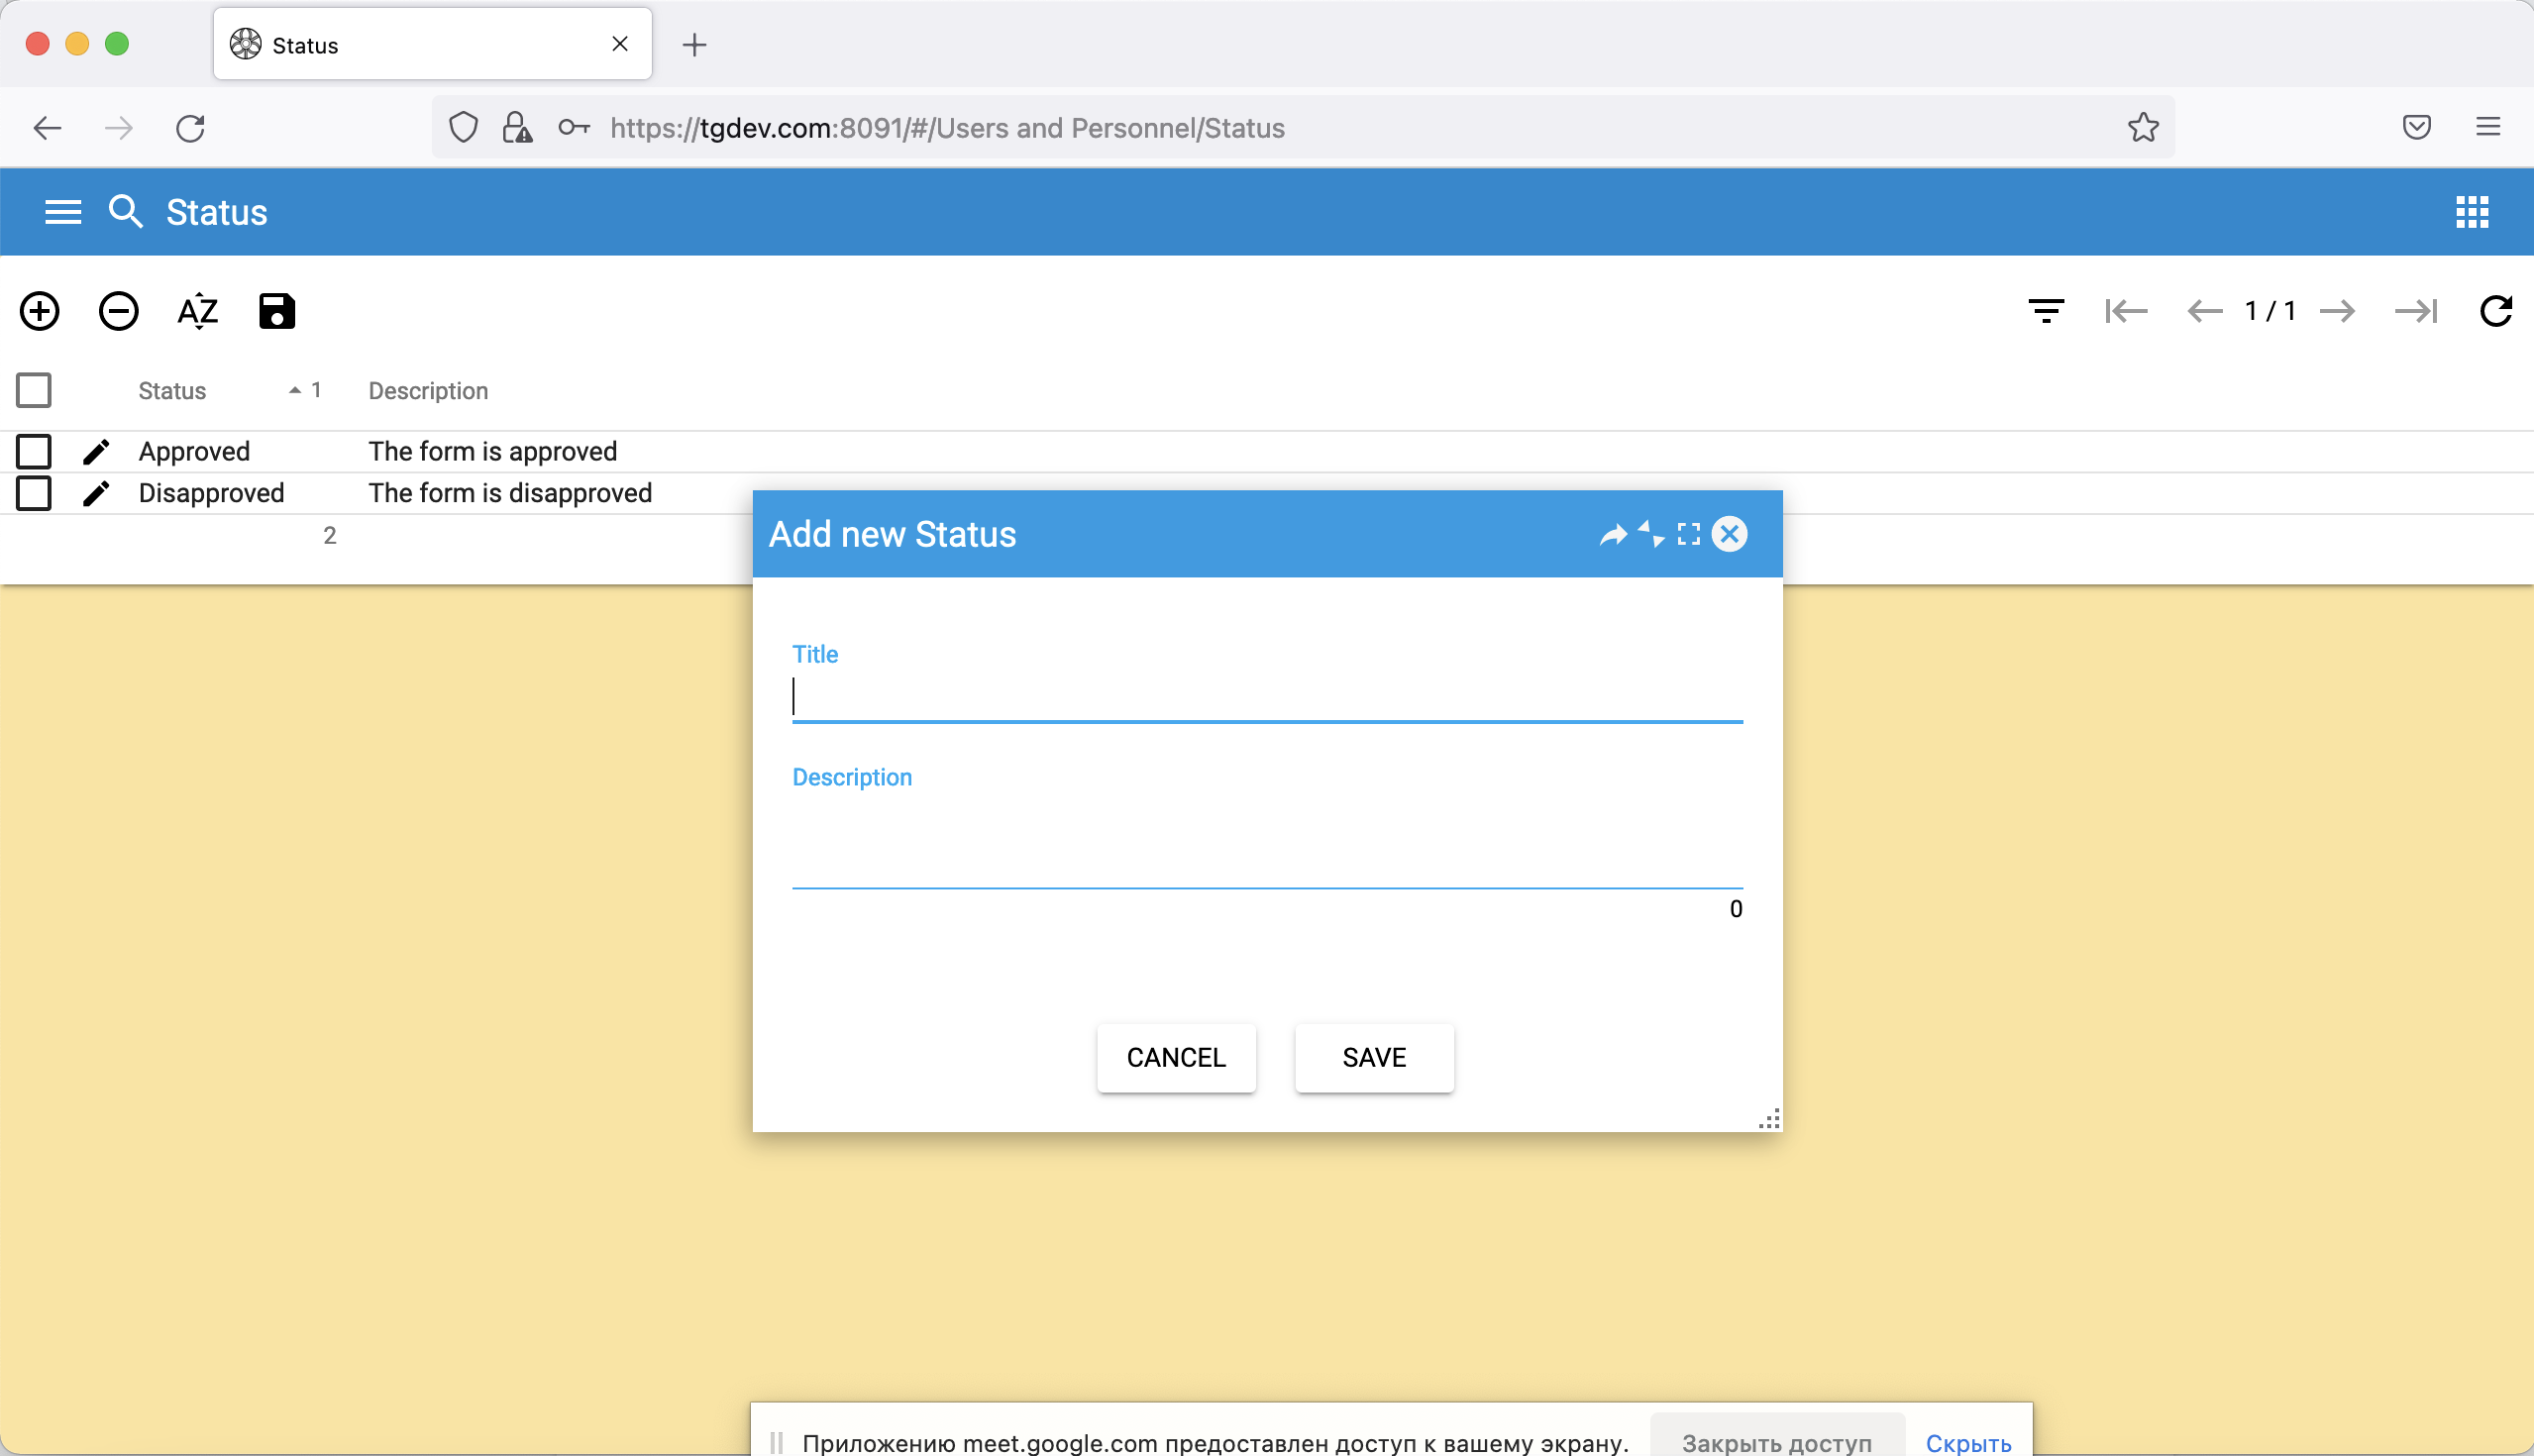
\includegraphics[width=0.95\linewidth]{sections/personnel/images/16.png}
\caption{Status creation.}\label{sections/personnel/images/16}
\end{figure}

\newpage
Users can also search for existing statuses either by specifying title, which is auto-completed, or description, or both, as displayed on
\hyperref[sections/personnel/images/17]{Fig.~\ref*{sections/personnel/images/17}}.

\begin{figure}[!htbp]
\centering
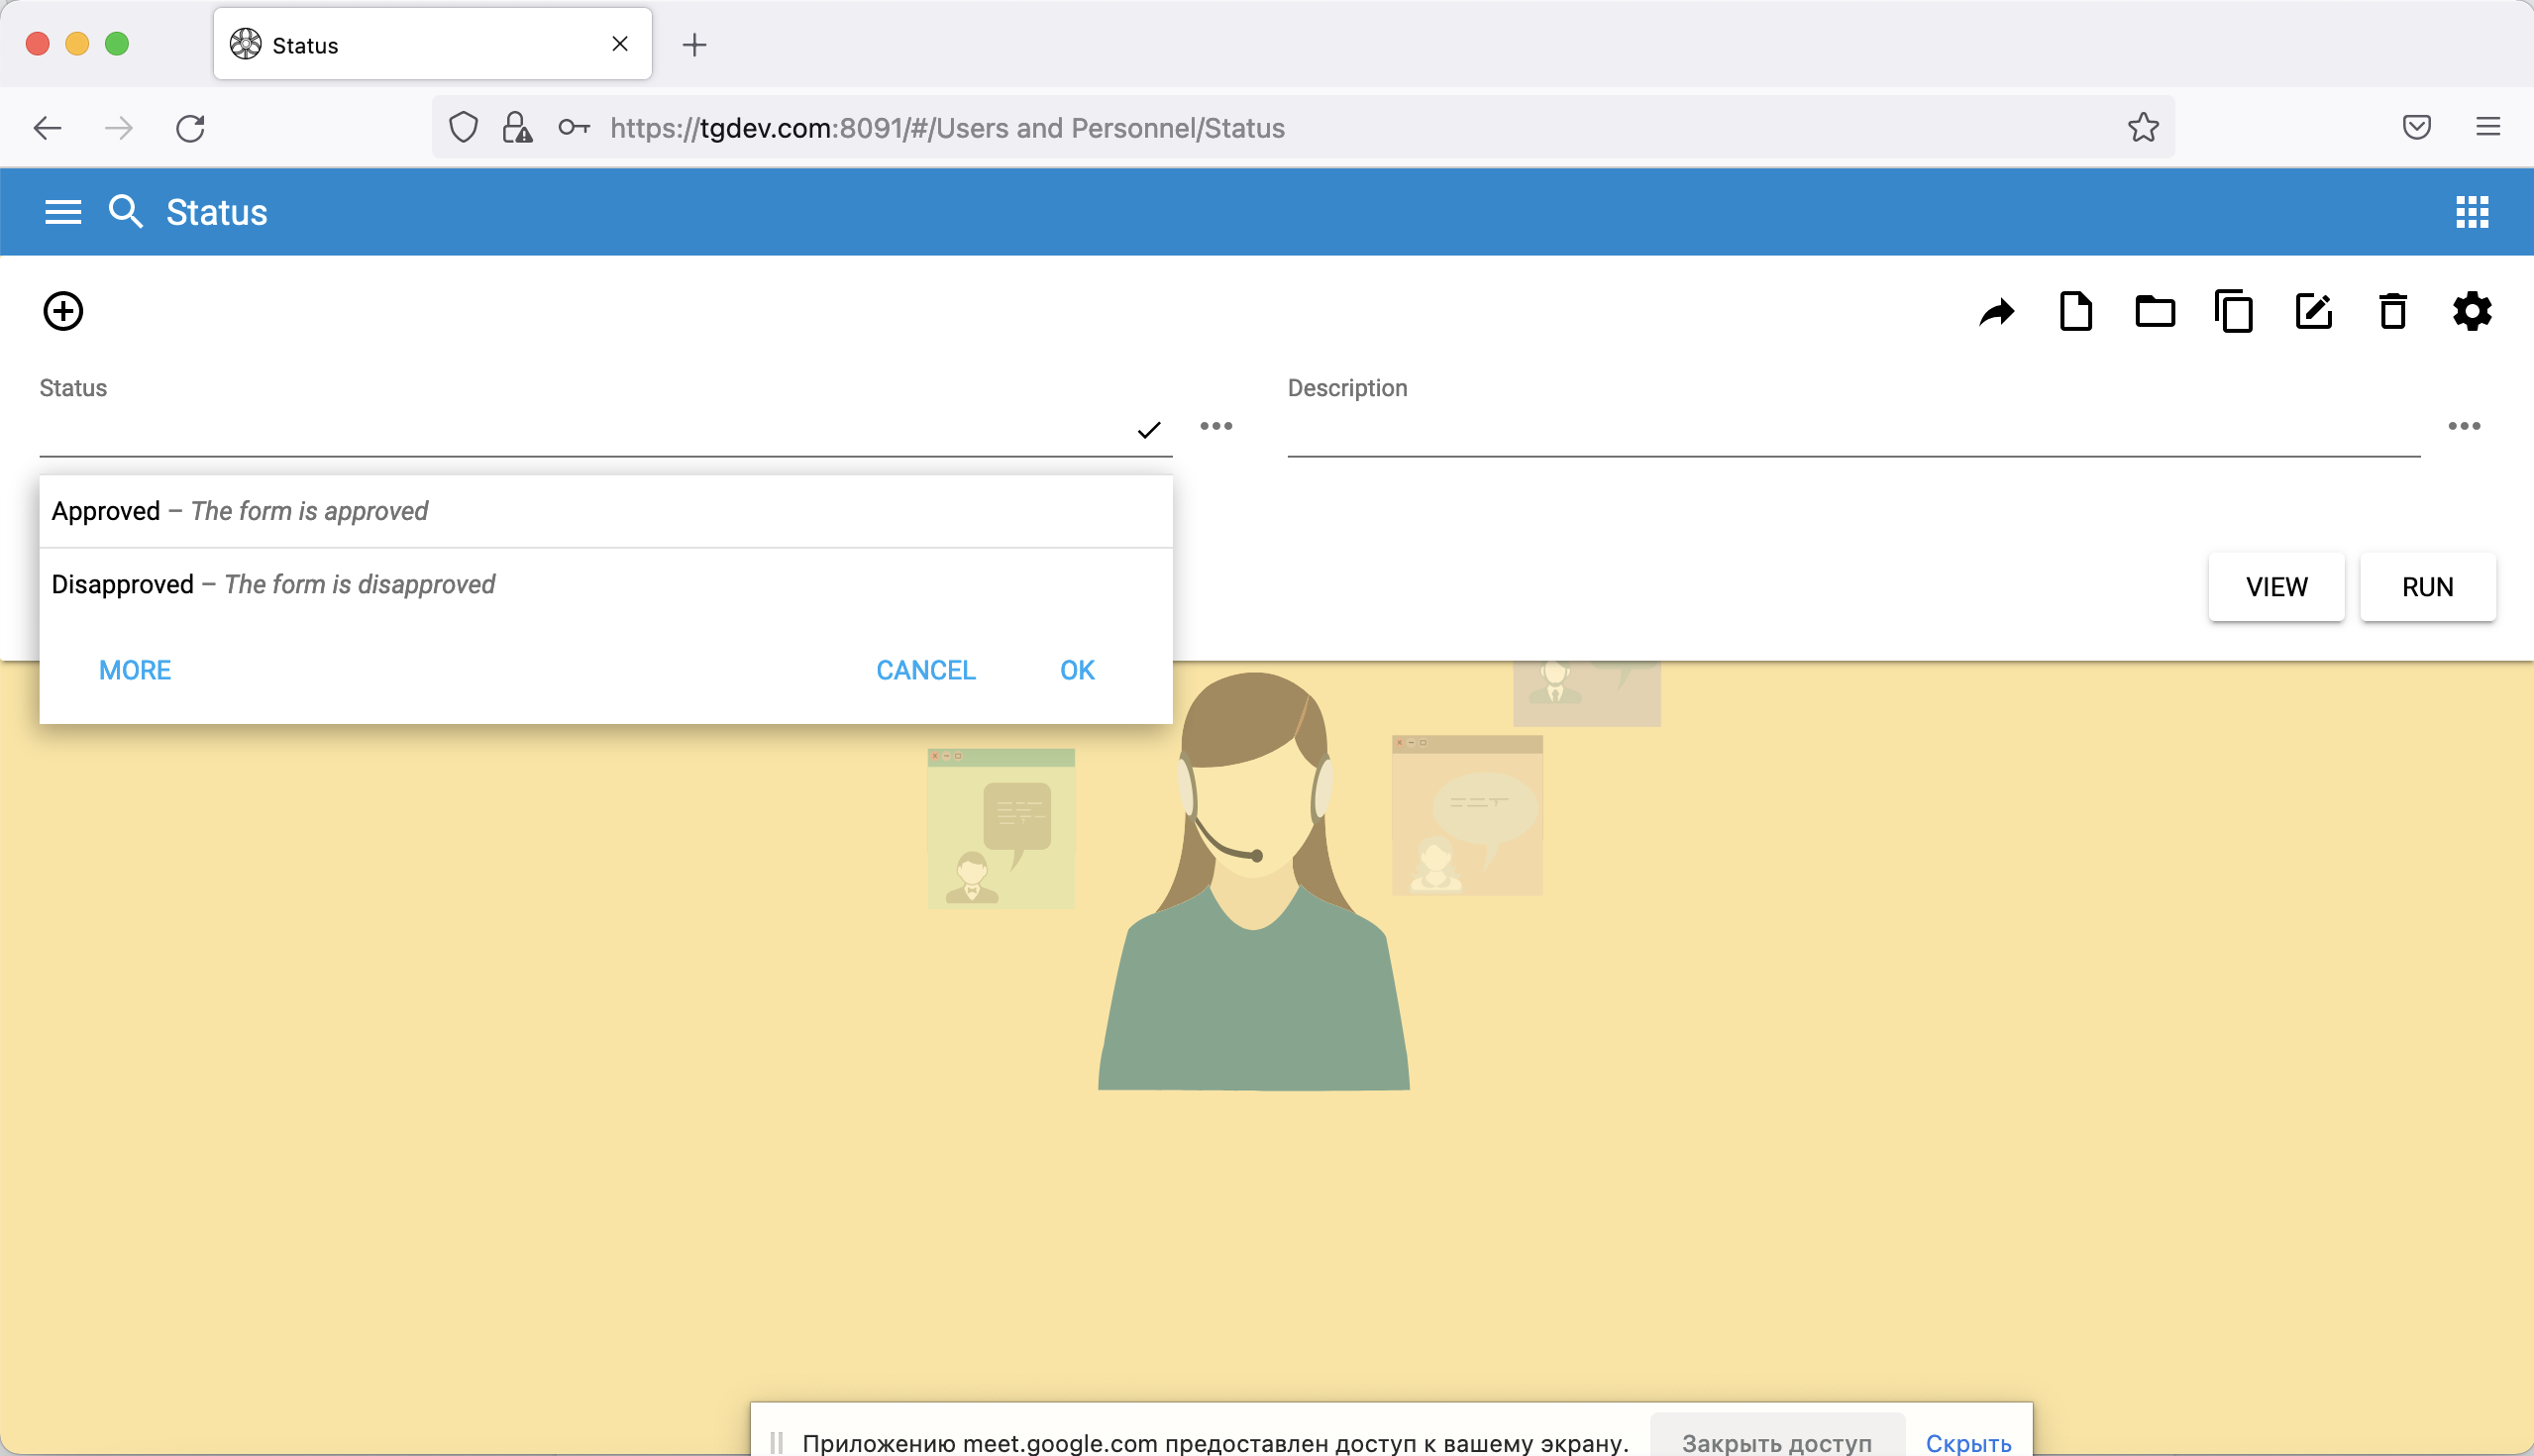
\includegraphics[width=0.95\linewidth]{sections/personnel/images/17.png}
\caption{Status search query.}\label{sections/personnel/images/17}
\end{figure}

\newpage
Search results are displayed along with title and description of the relevant statuses, as displayed on 
\hyperref[sections/personnel/images/18]{Fig.~\ref*{sections/personnel/images/18}}.

\begin{figure}[!htbp]
\centering
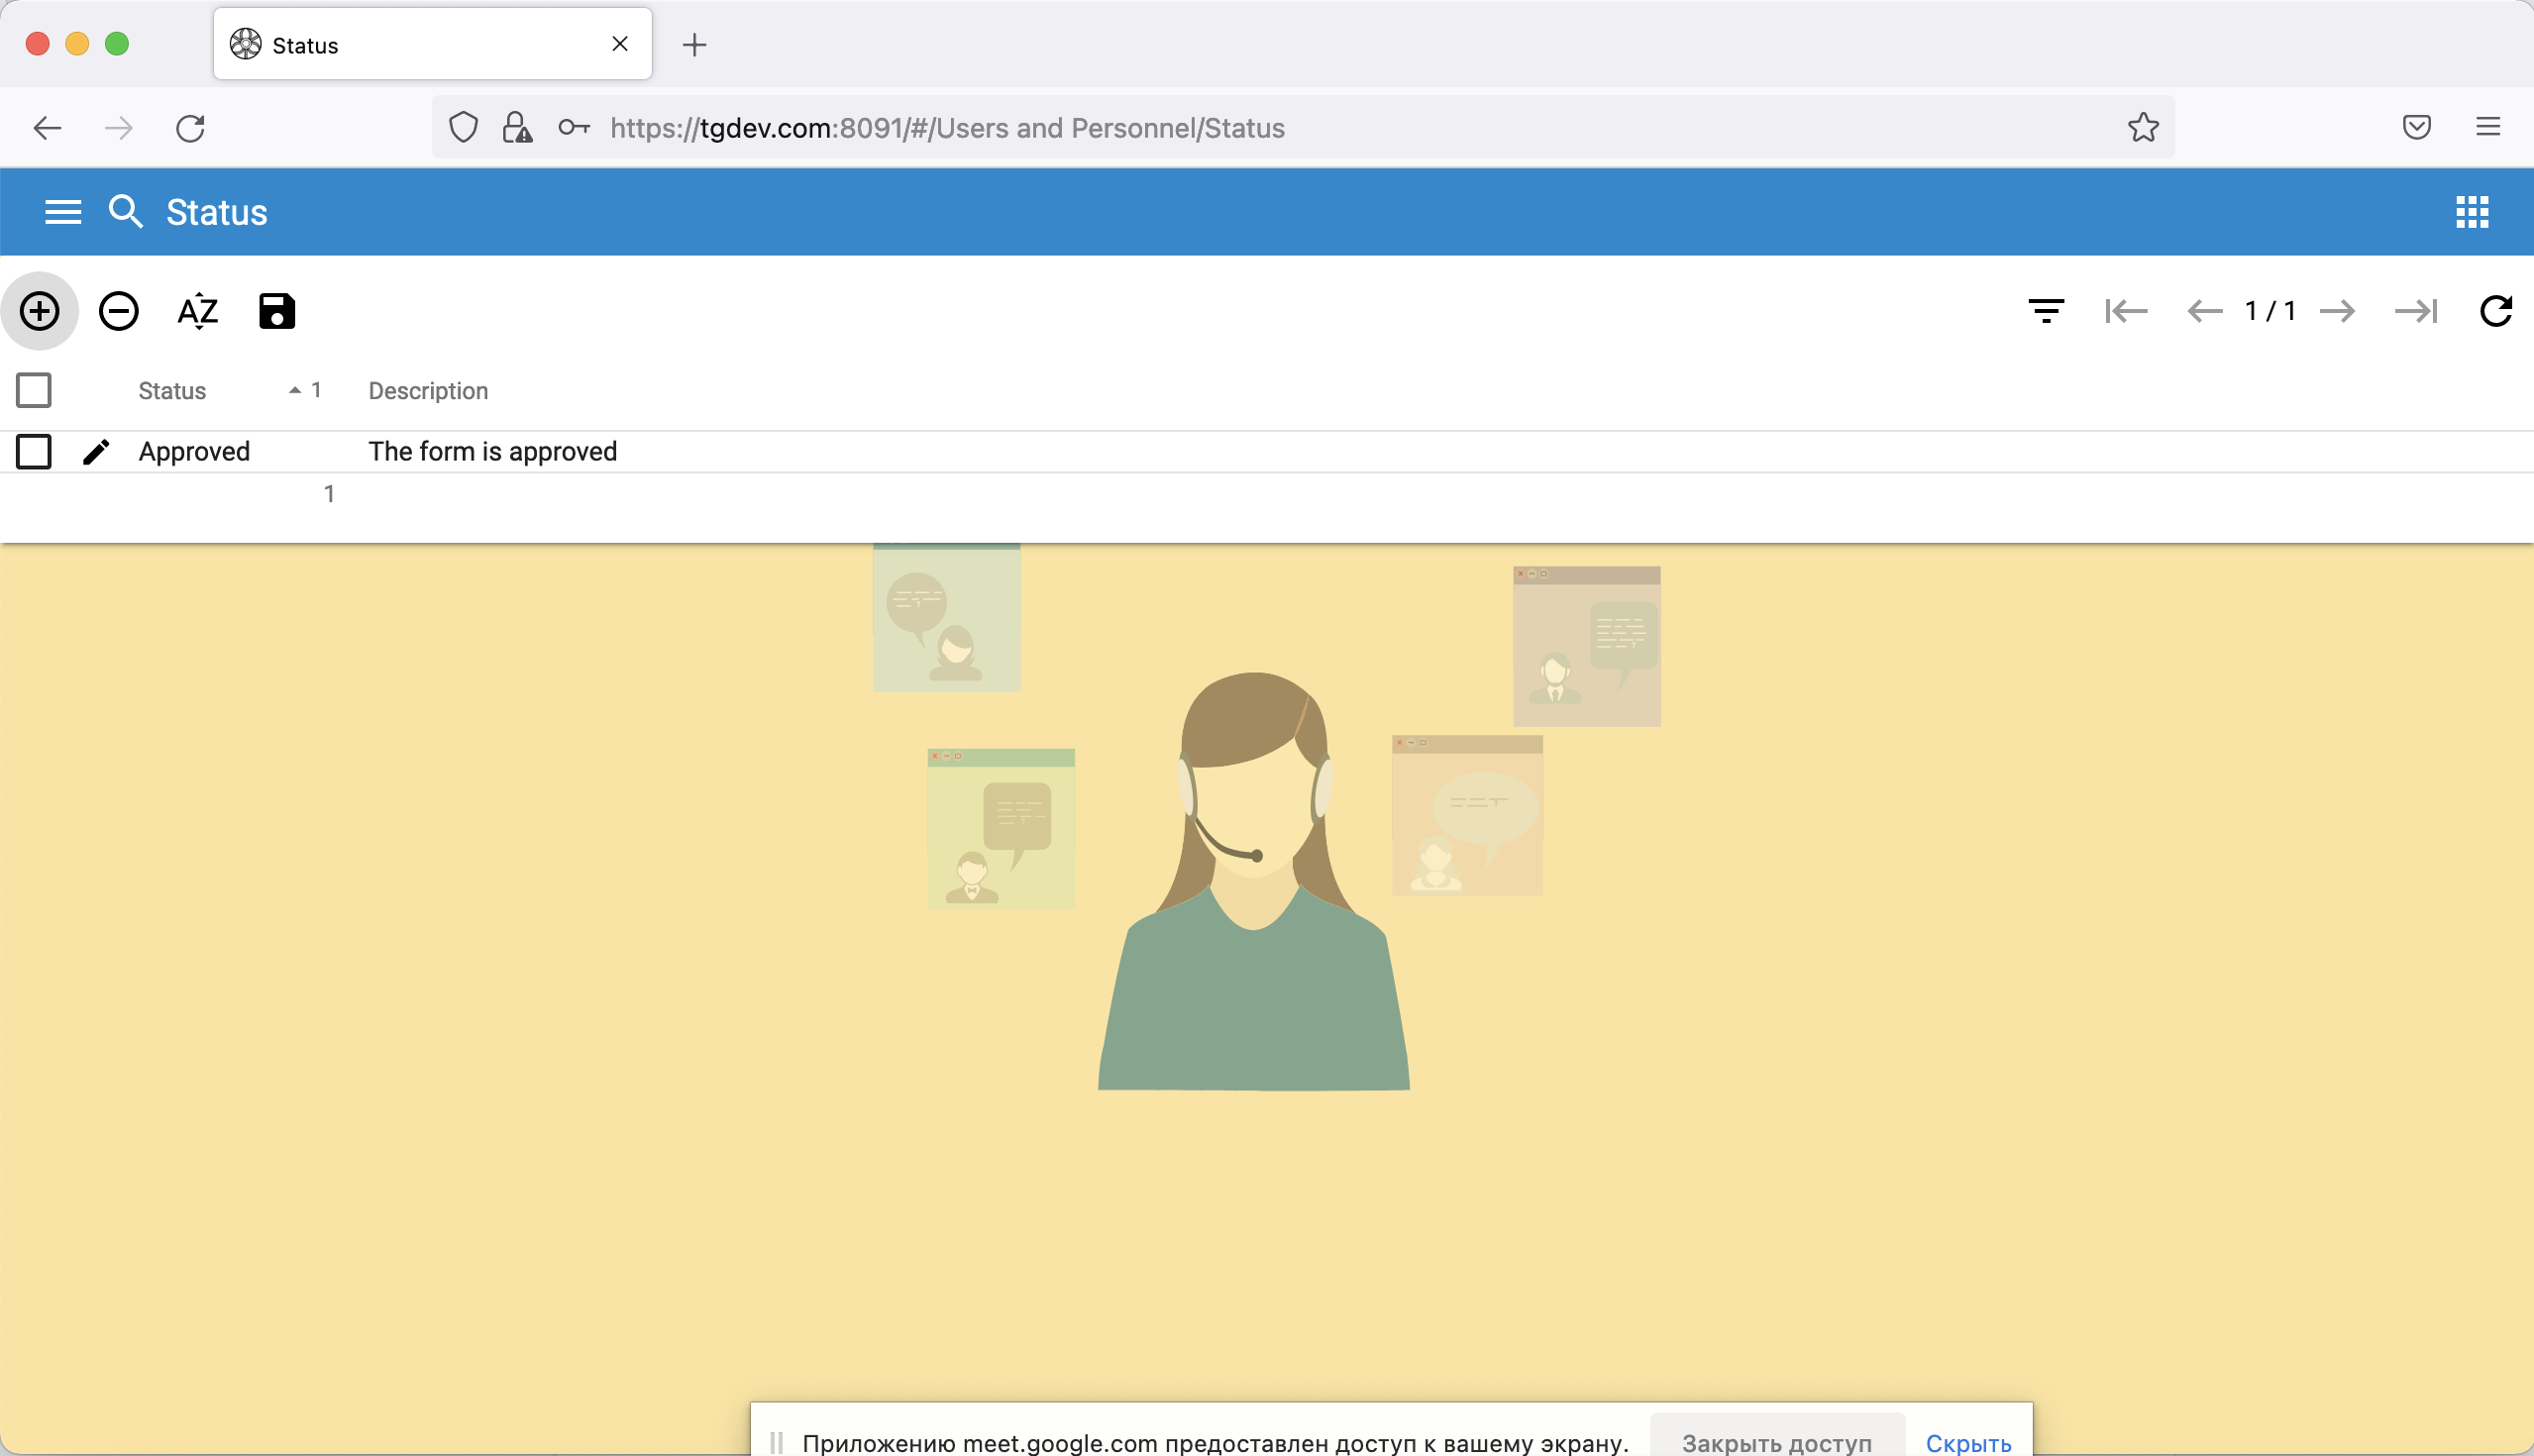
\includegraphics[width=0.95\linewidth]{sections/personnel/images/18.png}
\caption{Status search results.}\label{sections/personnel/images/18}
\end{figure}

\newpage
Users can edit existing statuses. As displayed on \hyperref[sections/personnel/images/19]{Fig.~\ref*{sections/personnel/images/19}}, users can edit title, and description of the specific status.

\begin{figure}[!htbp]
\centering
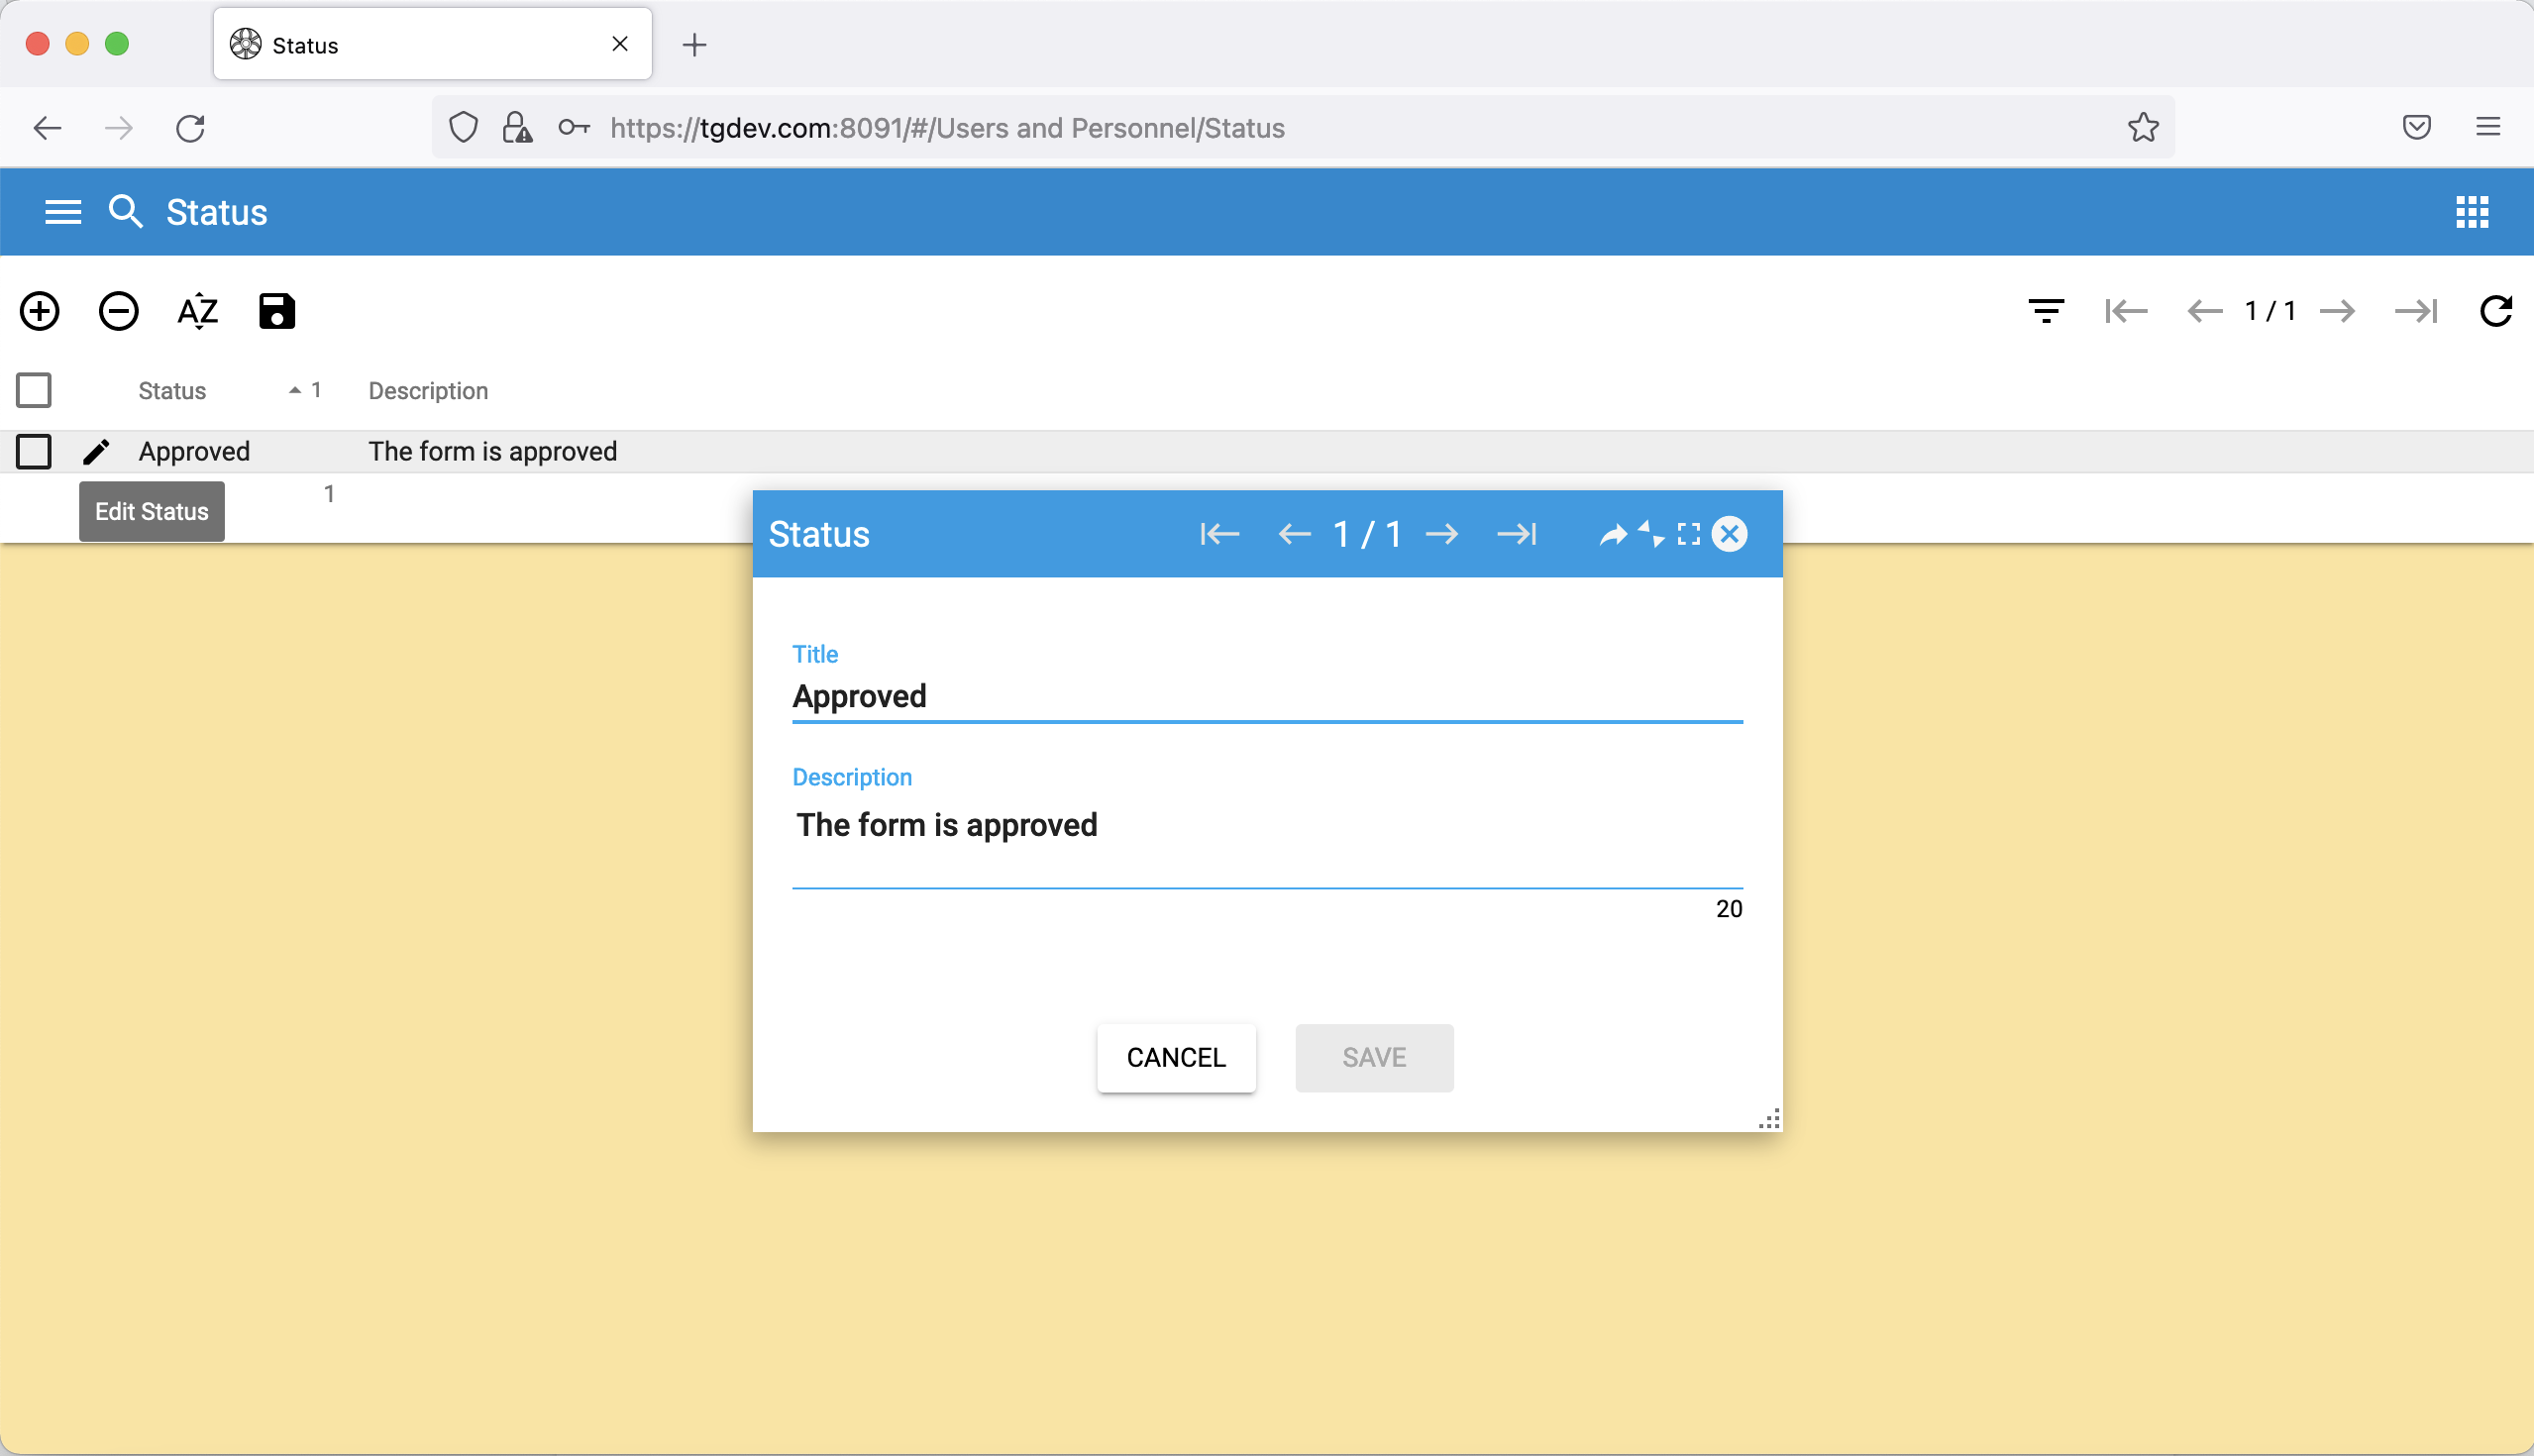
\includegraphics[width=0.95\linewidth]{sections/personnel/images/19.png}
\caption{Status editing.}\label{sections/personnel/images/19}
\end{figure}

\newpage
\subsection{Person}

In order to perform registration and save information about workers, users can create persons. When creating a new person, users have to fill in his/her name and surname, email, phone number in format +38 (098) 765 4321 (optional) and activity status, as displayed on \hyperref[sections/personnel/images/fig2]{Fig.~\ref*{sections/personnel/images/fig2}}.

\begin{figure}[!htbp]
\centering
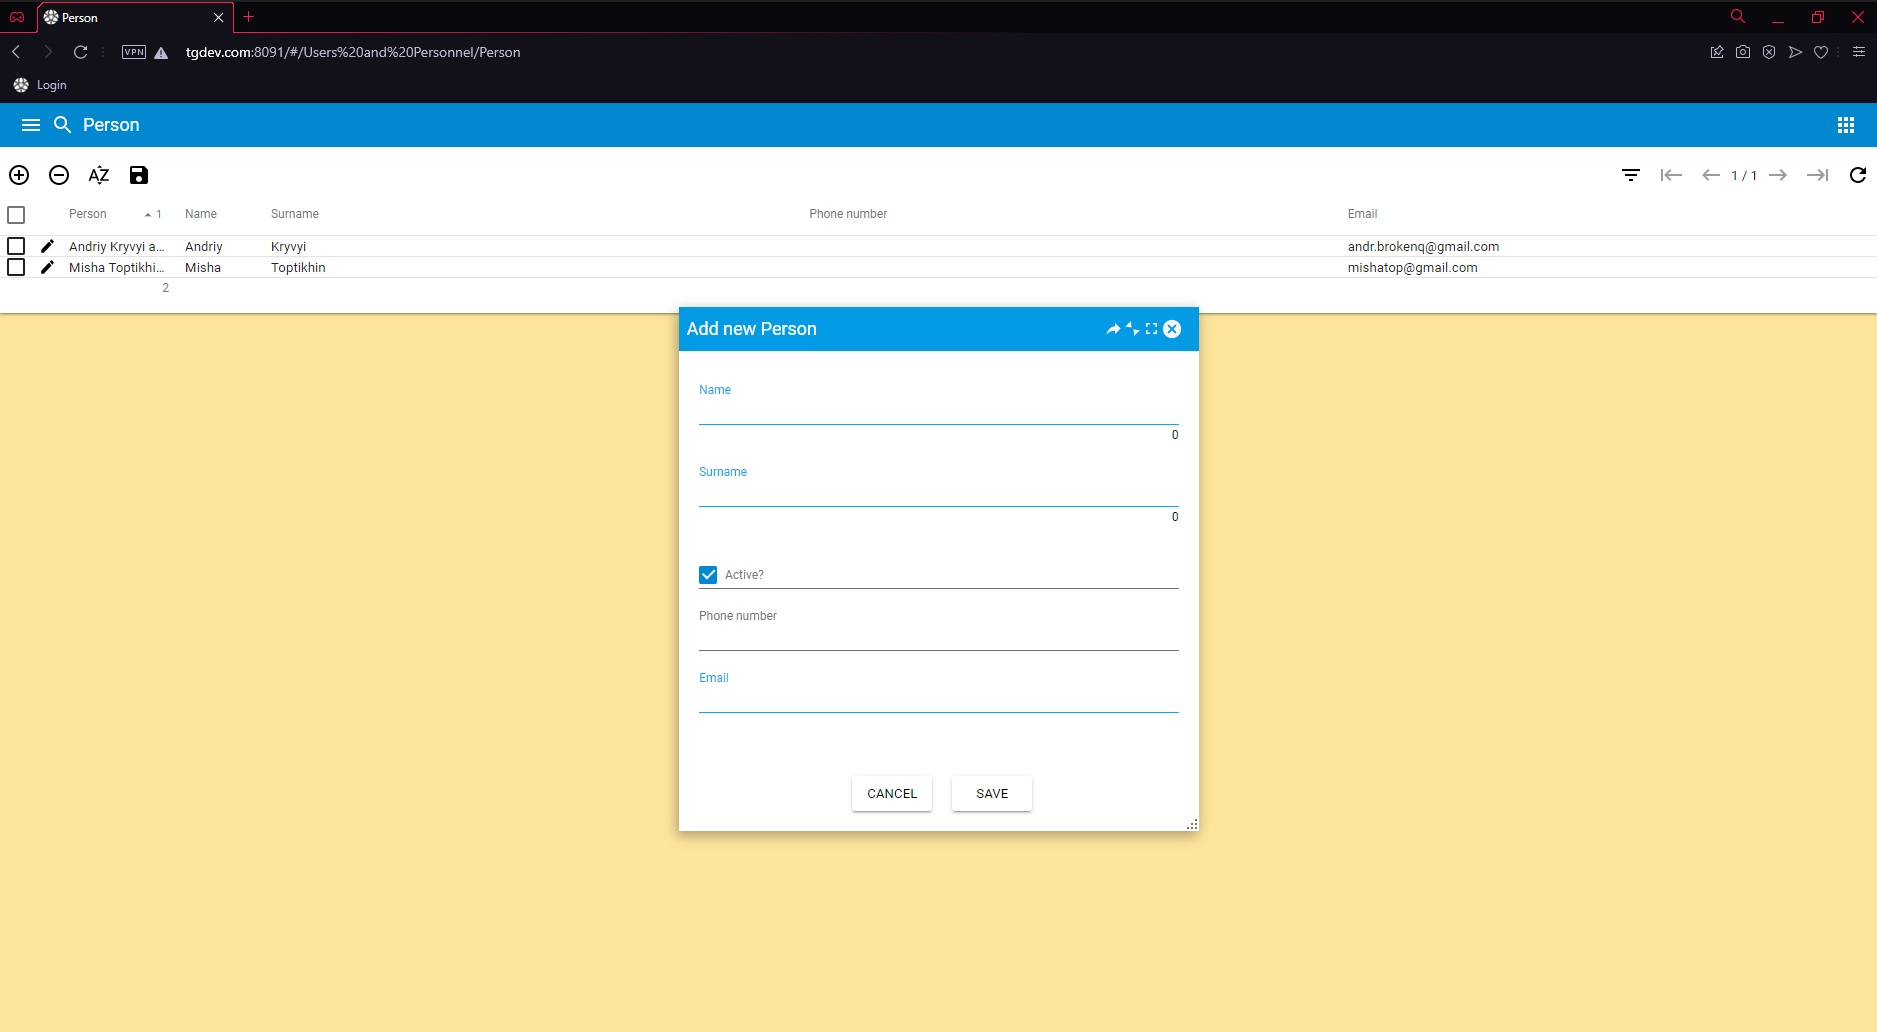
\includegraphics[width=0.95\linewidth]{sections/personnel/images/fig2.jpg}
\caption{Person creation.}\label{sections/personnel/images/fig2}
\end{figure}

\newpage
Users can search for existing persons either by specifying name, surname, or email, or phone number or activity status, or all of them as displayed on \hyperref[sections/personnel/images/fig1]{Fig.~\ref*{sections/personnel/images/fig1}}.

\begin{figure}[!htbp]
\centering
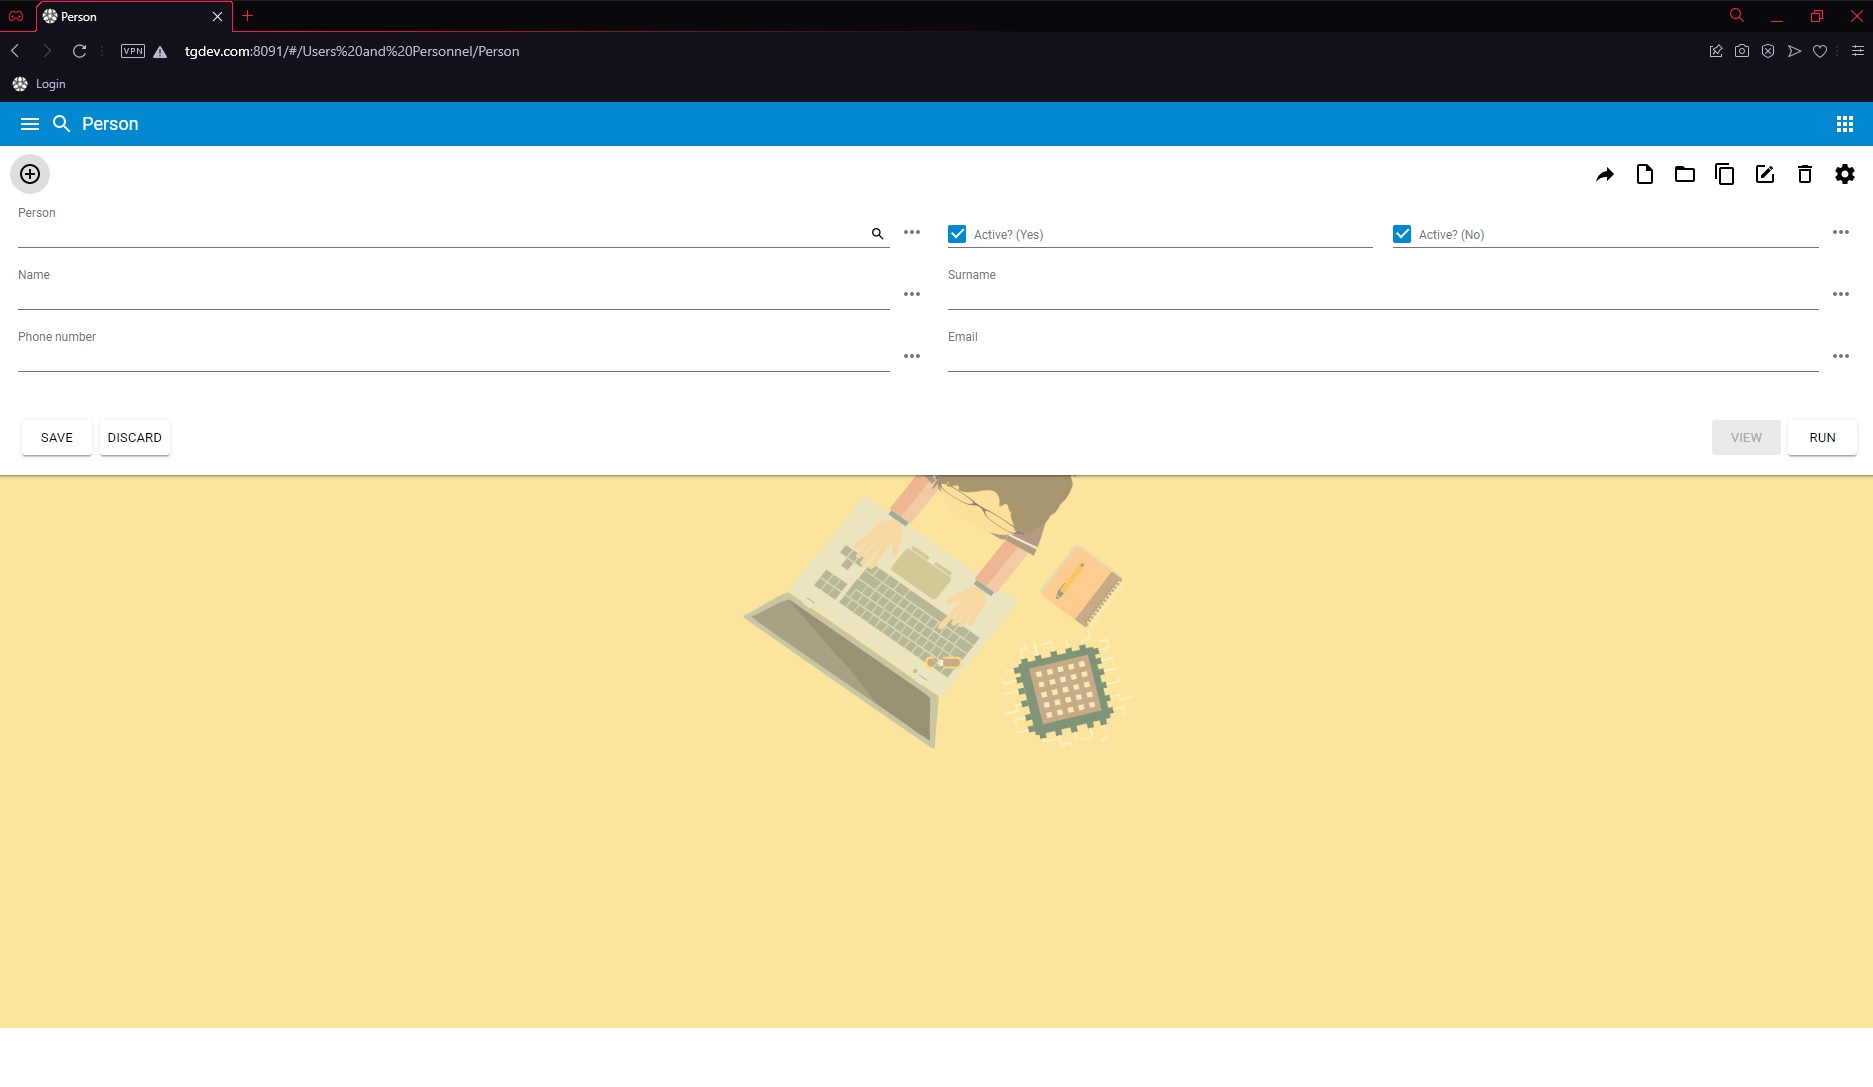
\includegraphics[width=0.95\linewidth]{sections/personnel/images/fig1.jpg}
\caption{Person search.}\label{sections/personnel/images/fig1}
\end{figure}

\newpage
Users can edit existing persons. On the ‘Main’ tab, displayed on \hyperref[sections/personnel/images/fig3]{Fig.~\ref*{sections/personnel/images/fig3}}, users can edit the name, surname, phone number, email and activity status of the specific person.

\begin{figure}[!htbp]
\centering
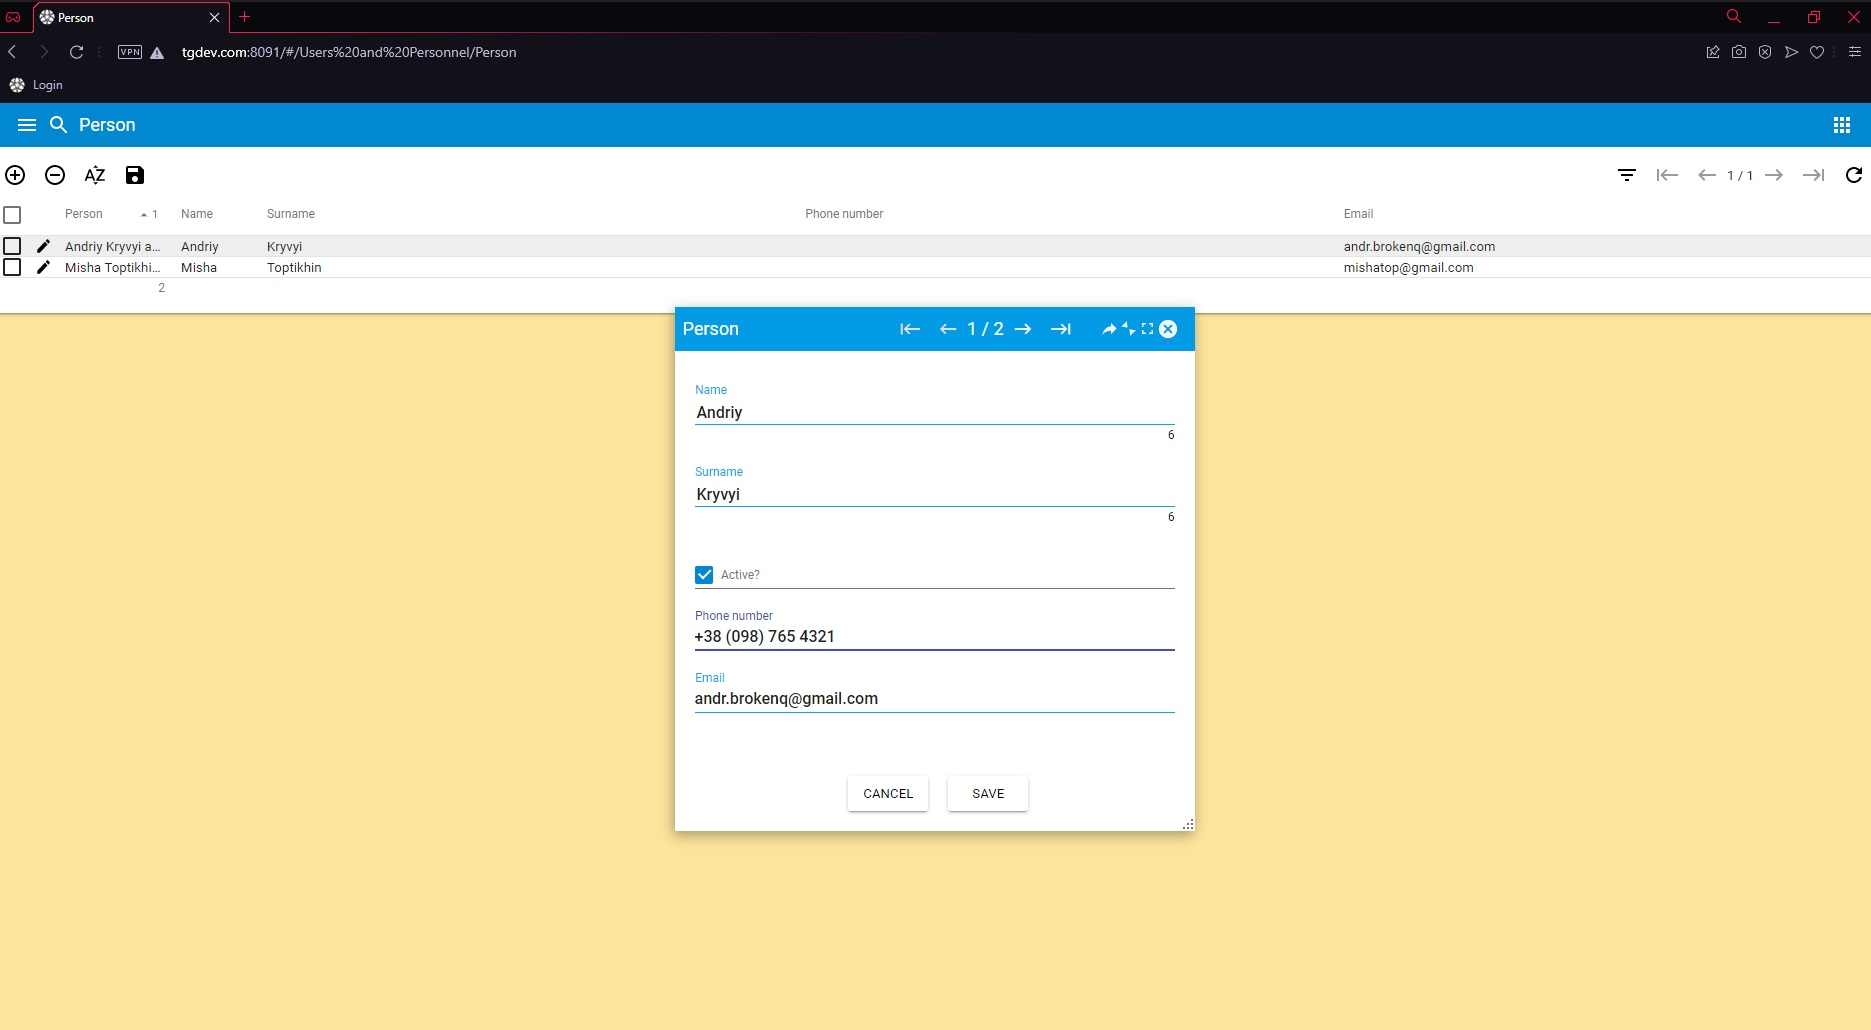
\includegraphics[width=0.95\linewidth]{sections/personnel/images/fig3.jpg}
\caption{Person editing.}\label{sections/personnel/images/fig3}
\end{figure}

\newpage
\subsection{Role}

In order to create and save roles, which will help to record the responsibility of workers, users can create roles. When creating a new role, users have to fill in its title and description as displayed on
\hyperref[sections/personnel/images/fig5]{Fig.~\ref*{sections/personnel/images/fig5}}.

\begin{figure}[!htbp]
\centering
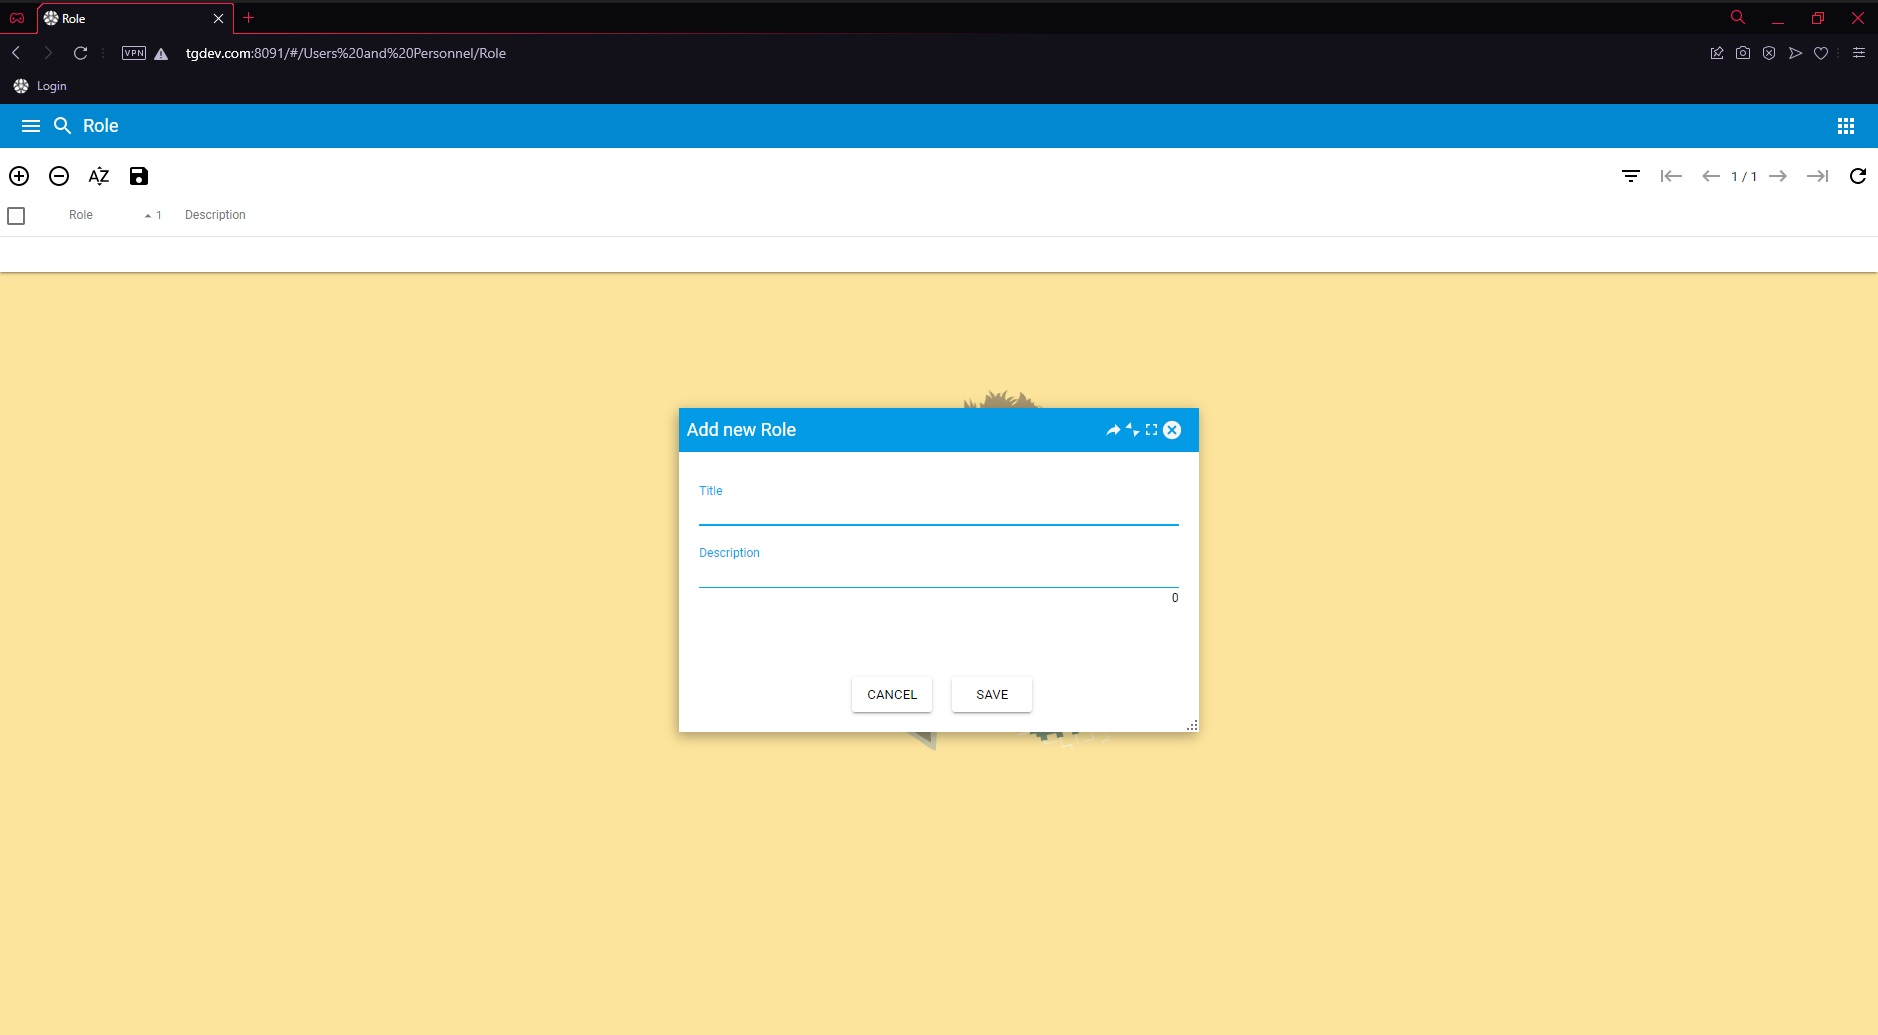
\includegraphics[width=0.95\linewidth]{sections/personnel/images/fig5.jpg}
\caption{Role creation.}\label{sections/personnel/images/fig5}
\end{figure}

\newpage
Users can search for existing roles either by specifying title, or description, or both as displayed on \hyperref[sections/personnel/images/fig4]{Fig.~\ref*{sections/personnel/images/fig4}}.

\begin{figure}[!htbp]
\centering
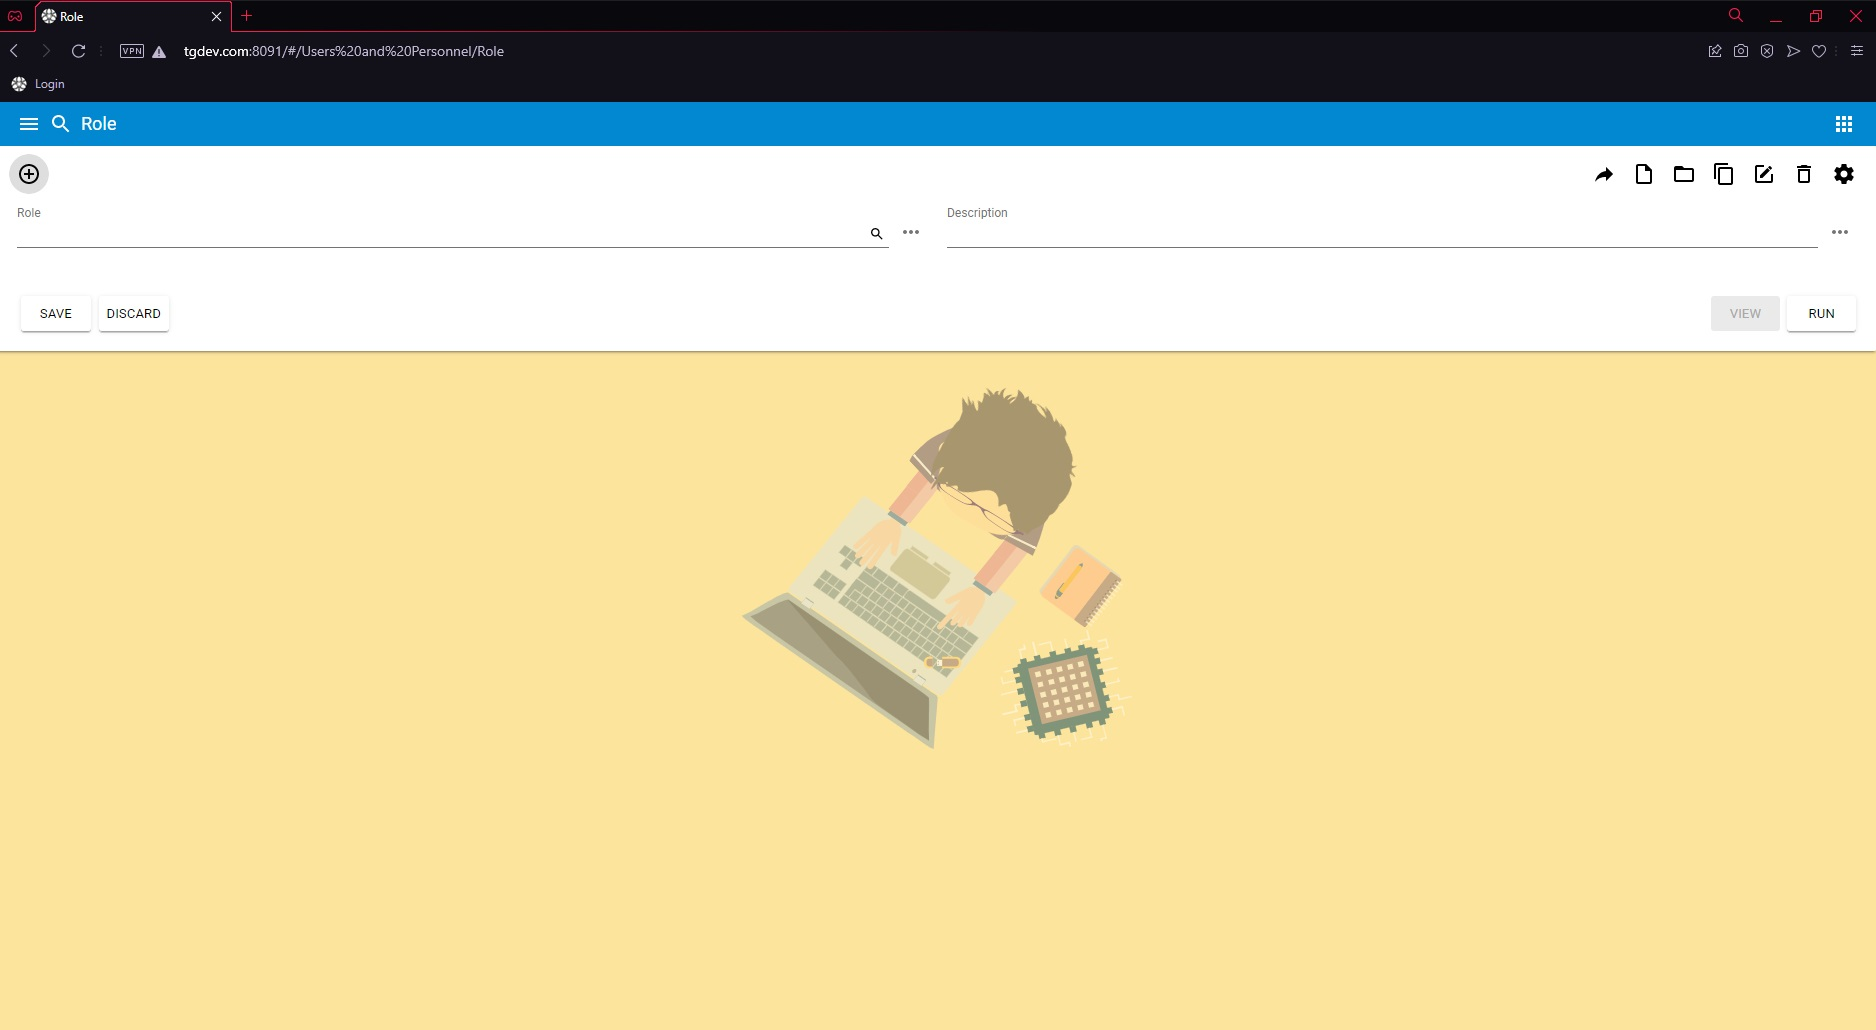
\includegraphics[width=0.95\linewidth]{sections/personnel/images/fig4.jpg}
\caption{Role search.}\label{sections/personnel/images/fig4}
\end{figure}

\newpage
Users can edit existing roles. On the ‘Main’ tab, displayed on \hyperref[sections/personnel/images/fig9]{Fig.~\ref*{sections/personnel/images/fig9}}, users can edit the title and description of the specific role.

\begin{figure}[!htbp]
\centering
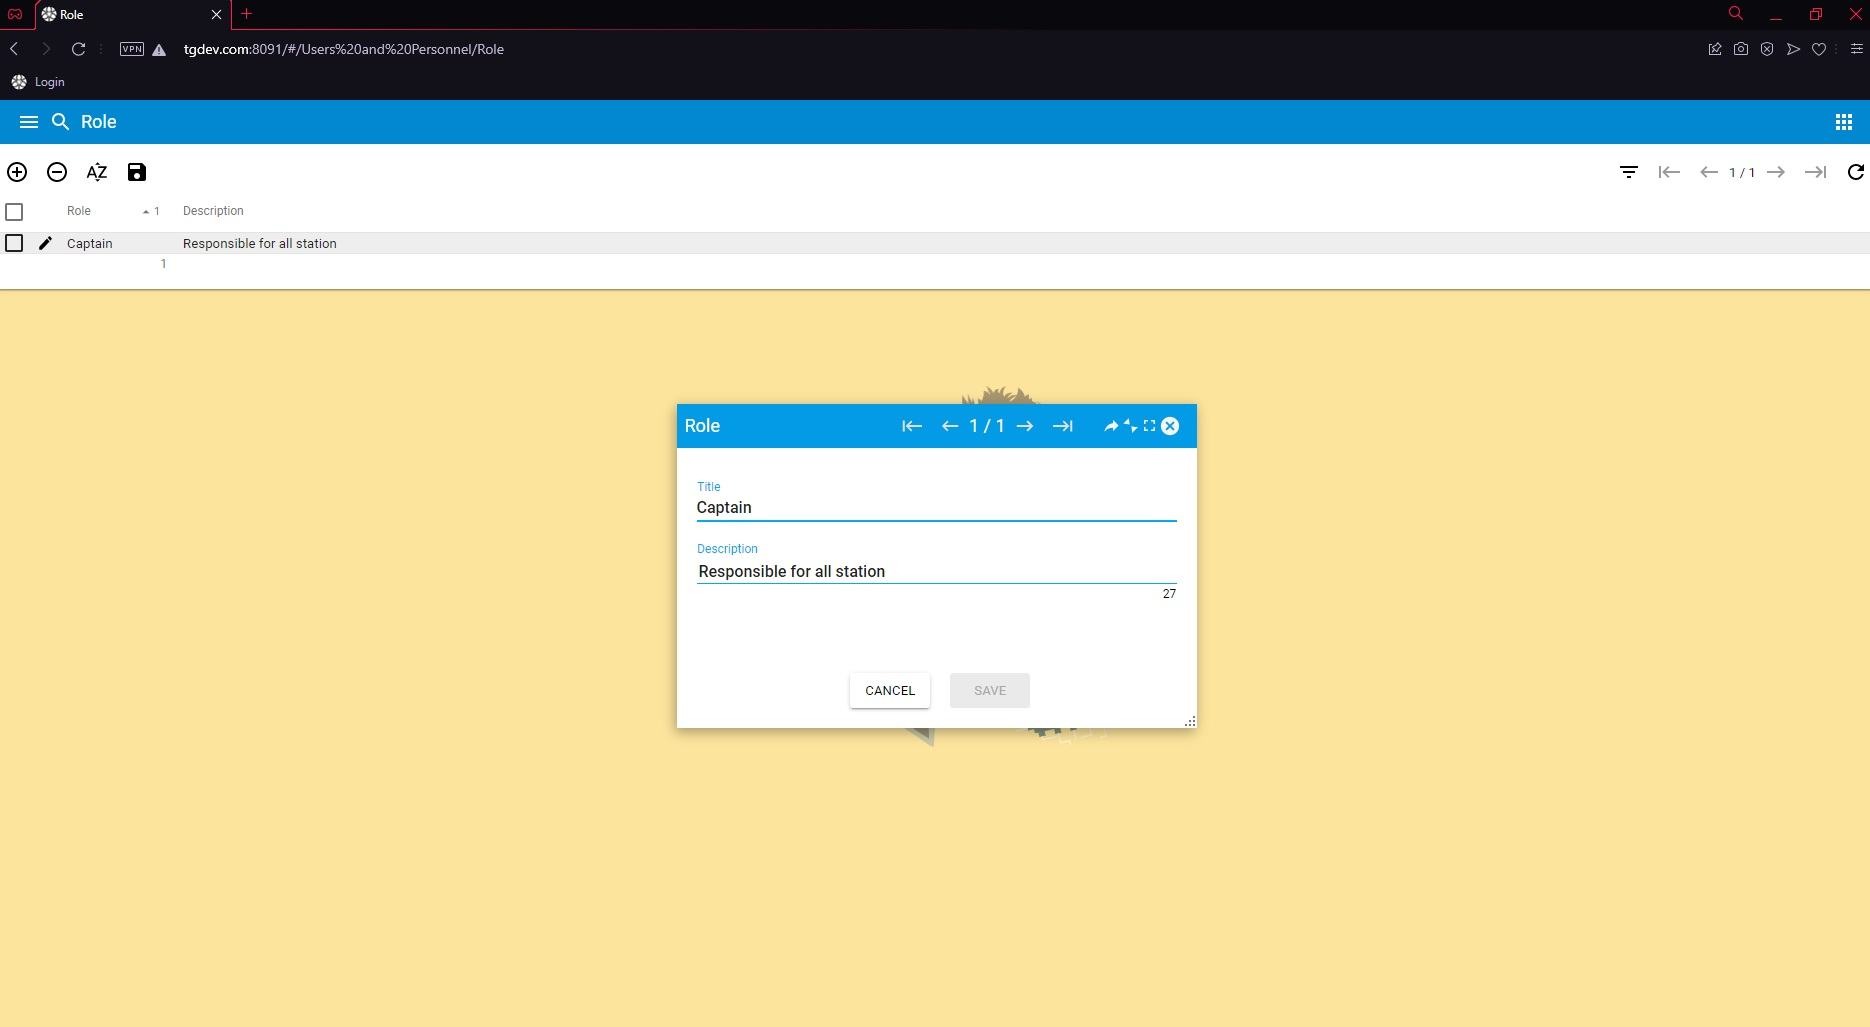
\includegraphics[width=0.95\linewidth]{sections/personnel/images/fig9.jpg}
\caption{Role editing.}\label{sections/personnel/images/fig9}
\end{figure}

\newpage
\subsection{Person role}

In order to assign a specific role to a worker at a specific date, users can create person role. When creating a new person role, users have to fill in the person, which is an autocomplete, role, which is also an autocomplete, and date when the role was assigned, as displayed on
\hyperref[sections/personnel/images/fig7]{Fig.~\ref*{sections/personnel/images/fig7}}.

\begin{figure}[!htbp]
\centering
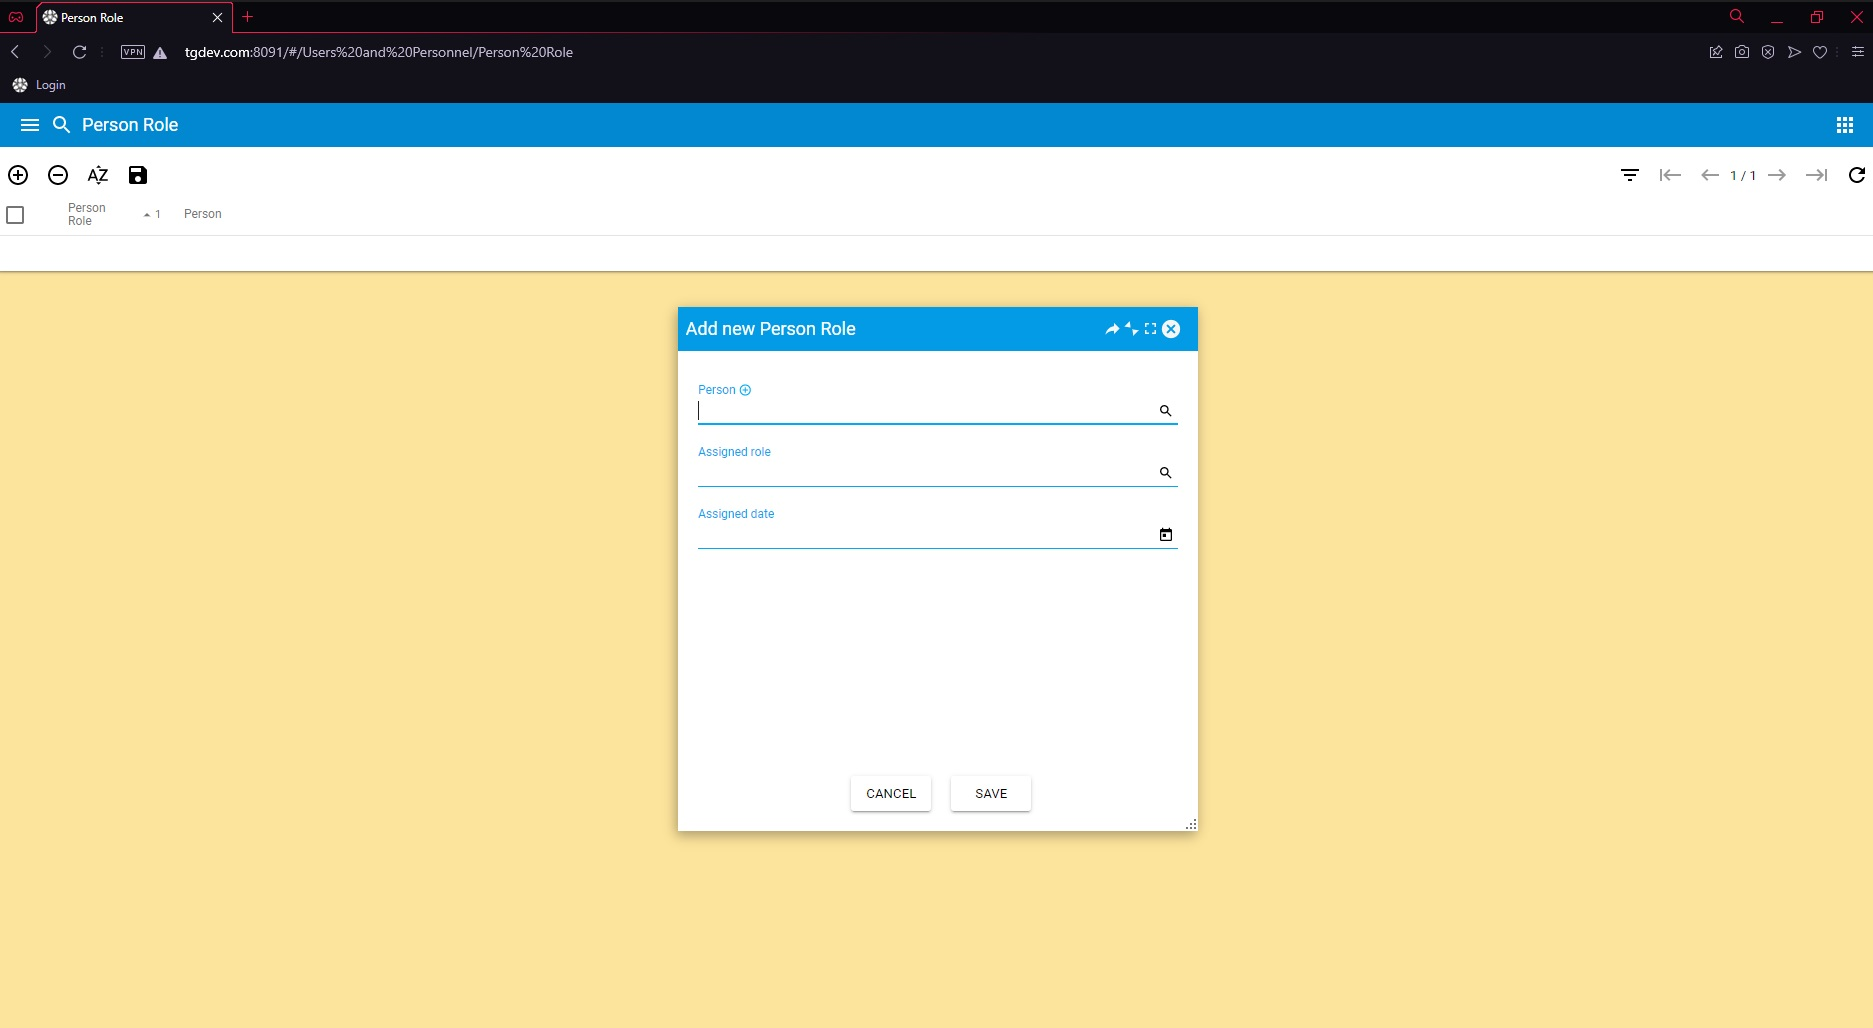
\includegraphics[width=0.95\linewidth]{sections/personnel/images/fig7.jpg}
\caption{Person role creation.}\label{sections/personnel/images/fig7}
\end{figure}

\newpage
Person and role fields have autocompletion so there is no need to type full person or role name by hand.

\begin{figure}[!htbp]
\centering
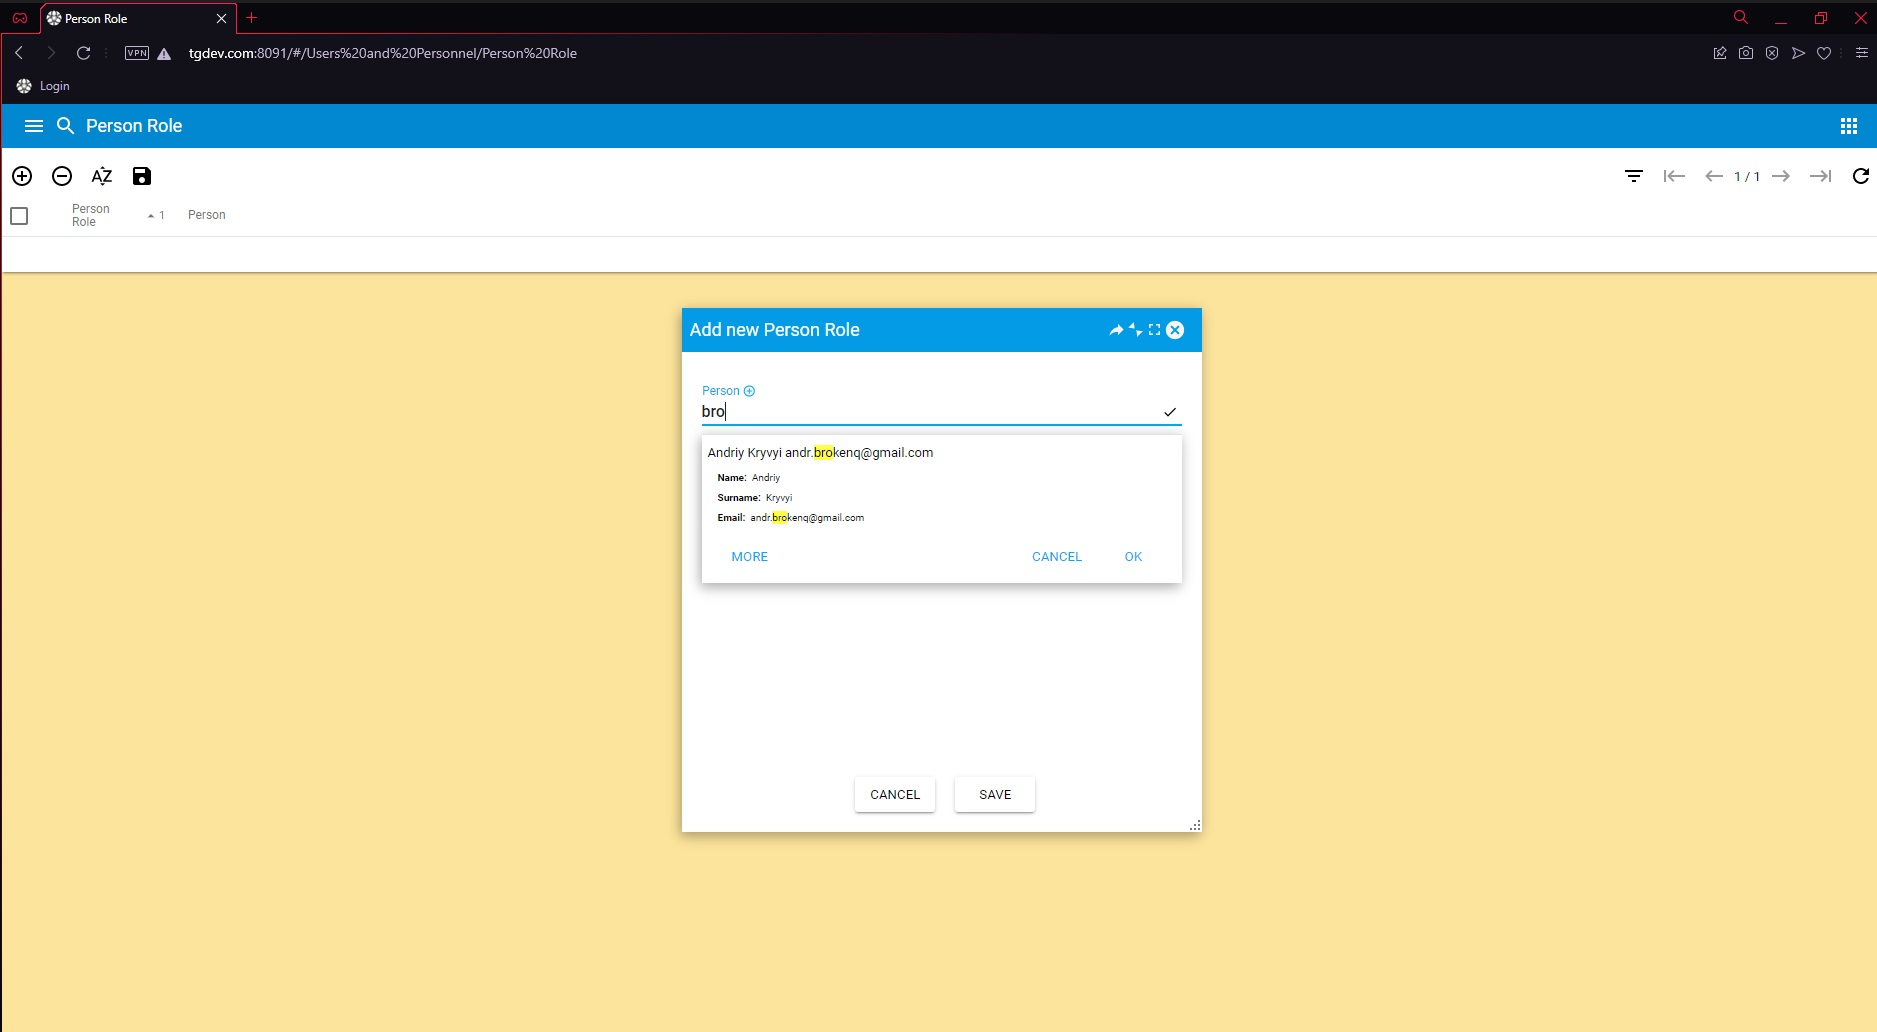
\includegraphics[width=0.95\linewidth]{sections/personnel/images/fig8.jpg}
\caption{Person field autocompletion.}\label{sections/personnel/images/fig8}
\end{figure}

\newpage
Users can search for existing person roles either by specifying person, or role, or date range, or all of them as displayed on \hyperref[sections/personnel/images/fig6]{Fig.~\ref*{sections/personnel/images/fig6}}.

\begin{figure}[!htbp]
\centering
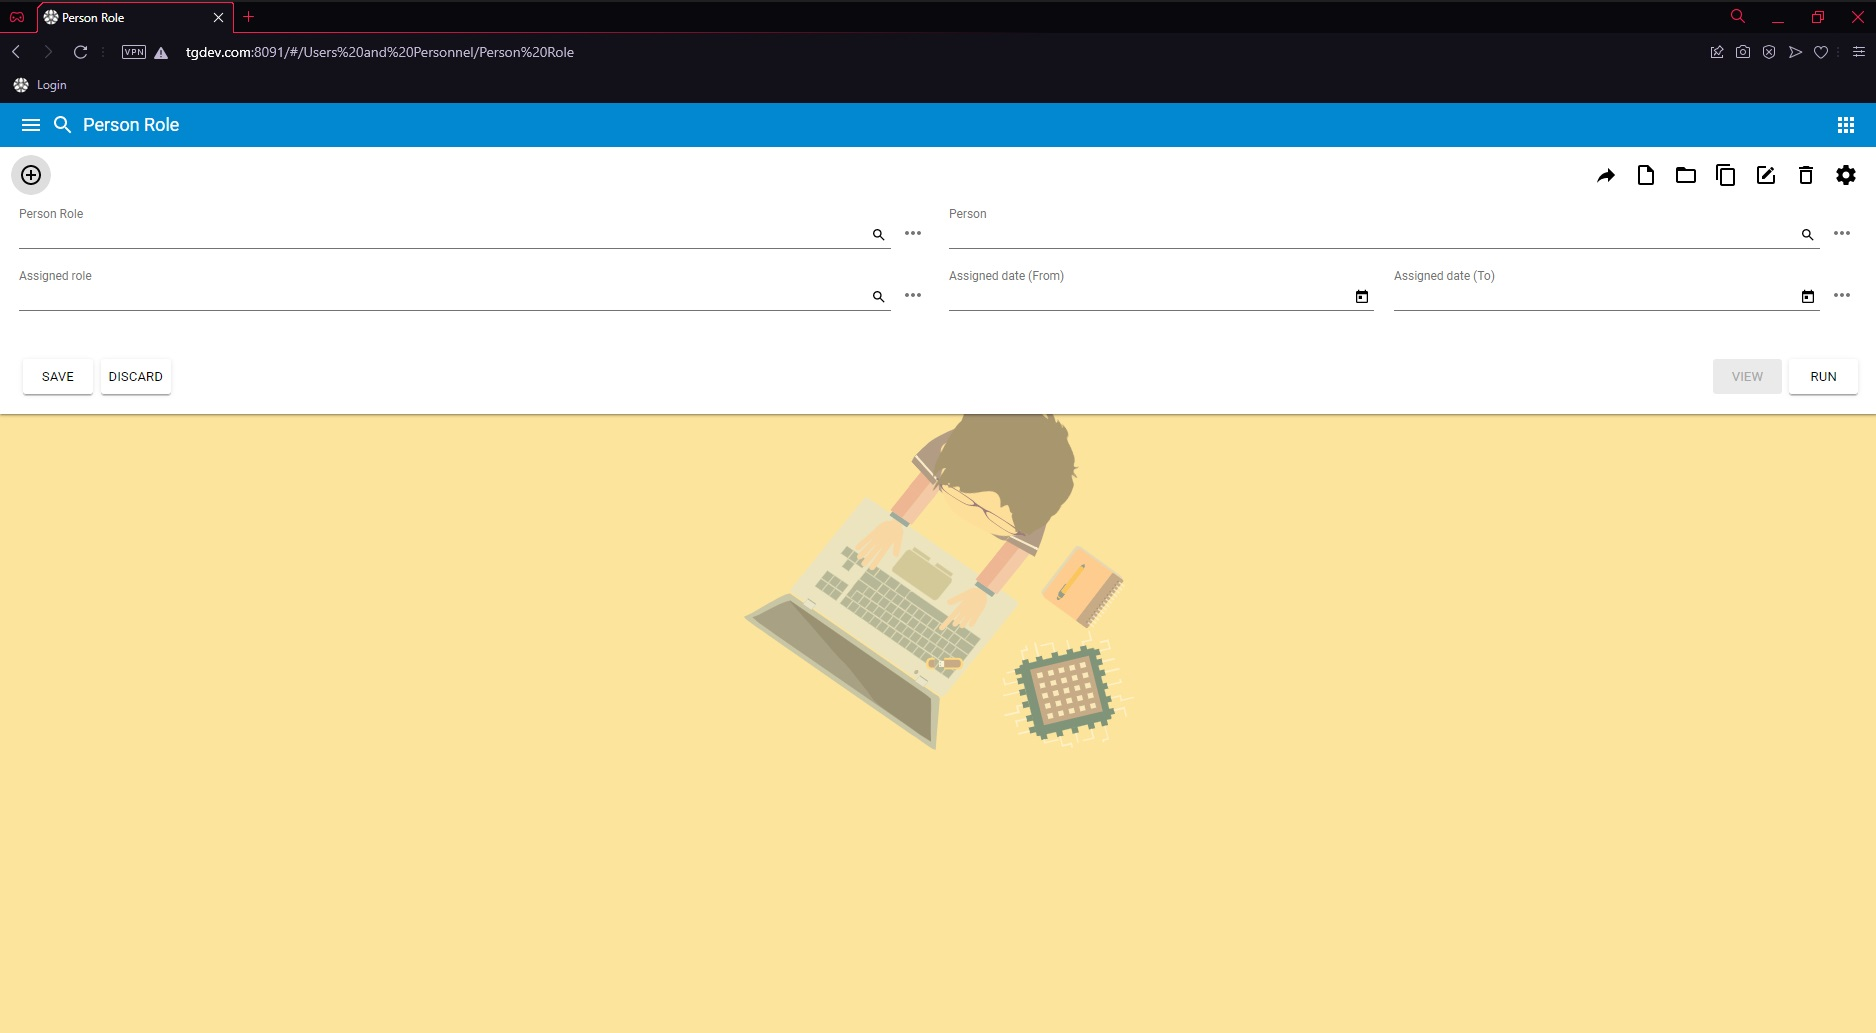
\includegraphics[width=0.95\linewidth]{sections/personnel/images/fig6.jpg}
\caption{Person role search.}\label{sections/personnel/images/fig6}
\end{figure}

\newpage
Users can edit existing person roles. On the ‘Main’ tab, displayed on \hyperref[sections/personnel/images/fig10]{Fig.~\ref*{sections/personnel/images/fig10}}, users can edit the person and role of the specific person role.

\begin{figure}[!htbp]
\centering
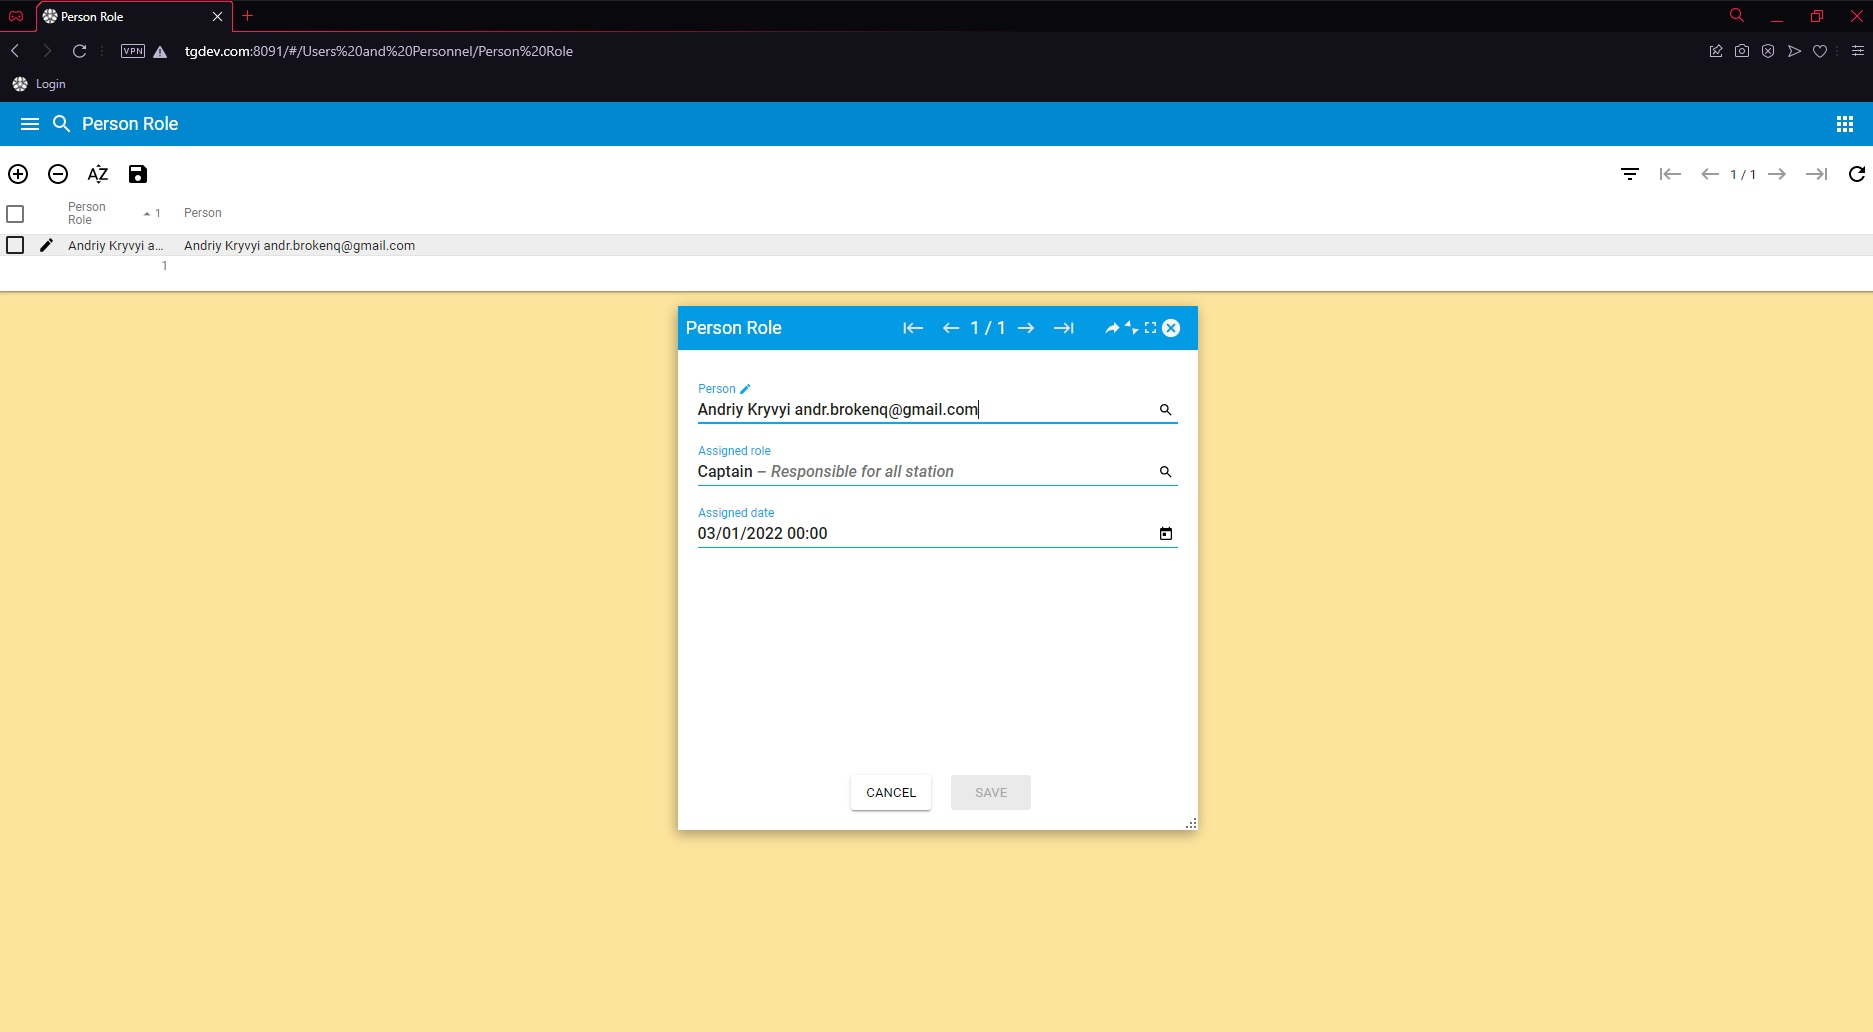
\includegraphics[width=0.95\linewidth]{sections/personnel/images/fig10.jpg}
\caption{Person role editing.}\label{sections/personnel/images/fig10}
\end{figure}
